%! Author = cspiller
%! Date = 16/11/2022

% Preamble
\documentclass[12pt, english]{article}

% Packages
% -- Typographic rules
\usepackage[english]{babel}
% -- Extended colors
\usepackage[dvipsnames]{xcolor}
% -- Embedded hyperlinks
\usepackage[colorlinks=true,linkcolor=BrickRed,citecolor=Fuchsia,pagebackref=true]{hyperref}
% -- Better text justification
\usepackage[nopatch=eqnum, auto=true, babel]{microtype}
% -- Images from file
\usepackage{graphicx}
\usepackage{svg}
% -- Better lists
\usepackage{enumitem}
% -- Bibliography format and access
\usepackage{natbib}
\usepackage{usebib}
% -- Glossary build
\usepackage[abbreviations]{glossaries-extra}
% -- Allow tables to cross pages
\usepackage{ltablex}
% -- Inline and display quotations
\usepackage[autostyle]{csquotes}
% -- Defines relative textsize commands
\usepackage{relsize}
% -- Used for AtBeginEnvironment hook
\usepackage{etoolbox}
% -- Adds extra symbols for quotations
\usepackage{textcomp}
% -- Adds better formatting for captions
\usepackage{caption}
% -- Visualise and change page layout
\usepackage{layout}
\usepackage{geometry}
% -- Code formatting
\usepackage{minted}
\setminted{
    linenos=true,
    autogobble,
}
\newenvironment{longlisting}{\captionsetup{type=listing}}{}

% Setup table column sizes (big and small)
\newcolumntype{z}{X}
\newcolumntype{s}{>{\hsize=.5\hsize}X}
% Setup page geometry
\geometry{
    a4paper,
    total={165mm,252mm},
    left=25mm,
    top=25mm,
}
% Makes display quotation smaller
\AtBeginEnvironment{quotation}{\smaller}
% Path to store image files for use in the document
\graphicspath{ {images/} }
% Import bibliography file
\bibinput{main}
% Glossary setup
\loadglsentries{glossary.tex}
\makeglossaries

% Document
\begin{document}
%    Title Page
    %! Author = cspiller
%! Date = 17/11/2022

\newcommand{\reportversion}{Interim}

\begin{titlepage}
    \begin{center}
        \vspace*{1cm}

        \huge
        \textbf{Spatialisation As A Service (SaaS)}

        \vspace{0.5cm}

        \large
        \reportversion~Project Report

        \vspace{1.5cm}

        \LARGE
        \textbf{Callum John Spiller}

        \vspace{1.5cm}

        \small
        Programme of study:\\
        \textbf{BSc FT Computer Science (Apprenticeship)}

        \vspace{1cm}

        Supervisor:\\
        \textbf{Johann Pauwels}

        \vfill

        \footnotesize
        Final Year\\
        Undergraduate Project 2022/23

        \vspace{0.5cm}
        
\includegraphics[width=0.4\textwidth]{qmlogo}
        \vspace{0.5cm}

        School of Electronic Engineering and Computer Science\\
        \today

    \end{center}
\end{titlepage}
    \newpage

%    Abstract Page
    \thispagestyle{plain}
\begin{center}
    \vspace{0.9cm}
    \textbf{Abstract}
\end{center}

Lorem ipsum dolor\ldots
    \newpage

%    Contents
    \tableofcontents
    \newpage

%    Glossary
    \printglossaries

%    Main Content
    %! Author = cspiller
%! Date = 17/11/2022
\thispagestyle{plain}
\newpage
\section{Introduction}\label{sec:introduction}
\subsection{Project Background}\label{subsec:project-background}
\normalsize

This project has been undertaken as a part of a degree apprenticeship with~\gls{sie}.\
As such, the final year engineering project for this author will consider the business domain of the sponsoring company.\\

With the release of the~\gls{ps5} in November 2020,~\gls{spatial_audio} technology has come into focus for~\gls{sie} as game developers seek to leverage the~\gls{tempest_3d_audio} espoused by the video game console.
In addition,~\gls{sie} is undergoing a shift to cloud-based infrastructure\footnote{like many other companies relying on web technology~\citep{cc_overview}} across the wider business in order to leverage the cost, flexibility, and reliability benefits that cloud technology affords~\citep{cc_overview}.\\

With respect to these developments in the business, this project seeks to engage both of these emergent technologies in order to address one of~\gls{sie}\textquotesingle s major~\glspl{sla} with a software solution.\\

\subsection{Problem Statement}\label{subsec:problem-statement}

The onboarding of~\glspl{pspartner} to the developer and publisher platforms managed by~\gls{sie} has been a targeted area for improvement within the company.
The primary challenge the business has faced in this area has been the reduction of friction in the process of getting~\glspl{pspartner} into the PlayStation ecosystem.\\

While the~\gls{pspartner} onboarding process has been automated and refined over time, this author argues that the ability for potential~\glspl{pspartner} to engage with and trial PlayStation's spatial audio technology is too restricted.\\

This project is based upon the hypothesis that, for a user who wishes to experiment with or experience~\gls{spatial_audio}, the barrier for entry is too high.
Engaging with a working demonstration of customisable~\gls{spatial_audio} requires a user to perform a significant amount of preparation on a local machine;
it demands a time commitment and pre-requisite technical knowledge that is far greater than is reasonable for an interested party to quickly evaluate what is possible.\\

Currently~\glspl{pspartner} who want to experiment with~\gls{tempest_3d_audio} must apply and order a~\gls{ps5} development kit, wait for it to arrive, set it up, then figure out how to engage with the~\glspl{api} provided by~\gls{sie}\textquotesingle s~\gls{devnet}.
This process is time-consuming and not optimal for a~\gls{pspartner} who wishes to get a quick insight into what is possible.\\

This project proposes an alternative solution where a~\gls{pspartner} who wishes to engage with the~\gls{spatial_audio} paradigm is able to experiment using a familiar audio file of their choosing.
The fact that the system will be accessible through a browser will mean that the~\gls{pspartner} will have much easier access, increasing the overall positive impression of the~\gls{pspartner} platform.\\

\subsection{Project Aims}\label{subsec:aims}

The primary aim of this project is to research, design, and engineer a web service that allows a user to easily experience~\gls{spatial_audio} in a way that reacts to their input.\\

The proposed workflow would allow a user to use a standard web browser\footnote{The project will most likely be designed for interaction through Chromium-based browsers and Firefox} to upload an audio file to a webpage and then receive back a new audio file that has rendered the stems from the original file into a \textquotesingle spatialised\textquotesingle ~format informed by \glspl{hrtf}.
All the audio processing would execute in \gls{aws} cloud environments to circumvent any real-world hardware requirements and challenges.\\

For vital information security reasons, the prototype produced as a part of this project will not feature any proprietary~\gls{sie} software and instead use only libraries that exist in the public domain.
As such, this prototype can be considered a~\gls{poc} where, if successful,~\gls{sie} software might be transplanted into the serverless pipeline.

\subsection{Project Objectives}\label{subsec:project-objectives}

In order to achieve the aims set out in Section~\ref{subsec:aims} the project must produce a number of deliverables:

\begin{enumerate}
    \item A project plan which outlines the timeline of both the research and development of the project
    \item A review of pertinent literature relating primarily to:
    \begin{itemize}
        \item Audio spatialisation
        \item Web audio \glspl{api}
        \item Cloud infrastructure (including those available from \gls{aws})
    \end{itemize}
    \item A review of existing stereo-to-ambisonic services and technologies.
    \item A functioning stereo-to-ambisonic serverless pipeline.
    \item A frontend that enables a user to interact with the conversion pipeline by uploading and downloading audio files, as well as setting parameters for conversion through a web~\gls{api}.
    \item A testing framework that supports iterative development.
    \item A report on user testing, including feedback from stakeholders.
    \item A review and analysis of how the produced system has met or missed the targets.
\end{enumerate}

\subsection{Research Questions}\label{subsec:research-questions}

In order to guide the research and development process of the proposed system, this report will seek to answer the following research questions:

\begin{enumerate}
    \item How is spatial audio rendered?
    \item Who might be interested in experiencing spatial audio, how might they do it, and why?
    \item What are the existing ways in which spatial audio can be experienced, and how accessible are they?
    \item Starting with a standard music file, what is the best way to demonstrate the capabilities of spatial audio rendering?
    \item How can intensive audio processing be performed in cloud environments?
    \item How might audio that is rendered in the cloud be delivered efficiently back to a web front-end?

\end{enumerate}
    %! Author = cspiller
%! Date = 17/11/2022

\thispagestyle{plain}
\newpage
\section{Literature Review}\label{sec:literature-review}

\normalsize

As outlined in~\ref{subsec:aims}, this project attempts to engage with cloud infrastructure, spatial audio processing, and web development frameworks.
To approach these topics thoroughly, this report performs a review of pertinent literature.
In doing so, this report considers and incorporates existing ideas in these fields while providing a foundation from which to answer the research questions listed in~\ref{subsec:research-questions}.

\subsection{Cloud Computing}\label{subsec:cloud-computing}

Ever since internet service providers began the commercialisation of cloud computing, it has become one of the major trends in the technology space~\citep{cc_overview}.
According to~\citet{cc_overview}, `cloud computing' is one of the most vague terms when it comes to the description of the technology on account of the breadth of its application

% TODO Continue from here - explain cloud concepts and benefits, downsides and challenges

s2\citep{cc_challenges}

Cloud computing technology is dominated by three major players, each with their own style of cloud services:
\begin{enumerate}
    \item Amazon's Web Services which began as a means of server virtualization~\citep{awsintro}
    \item Google's Cloud Platform, described by~\citet{cc_overview} as a technique-specific sandbox that calls itself a~\gls{paas}~\citep{googlecloudintro}
    \item Microsoft's Azure Network~\citep{azurefundamentals}
\end{enumerate}

% TODO describe current state of public cloud landscape and current capabilities of these platforms and effect on businesses



\subsection{Audio Spatialisation}\label{subsec:audio-spatialisation}
\subsubsection{Origins}

\citet{blauert_spatial} notes in their seminal text,~\textit{\usebibentry{blauert_spatial}{title}}, that: \textquote{human beings are primarily visually-orientated}, and that the other senses are less developed in comparison.
This difference has been mirrored in the history of scientific research.
\citet{wade_binaural} note that research in binaural hearing was developed later than binocular vision partially due to the difficulty in controlling the audio stimuli in experiments.
It was only later on that the concept of distinction between the~\textit{sound event} and the~\textit{auditory event} as influenced by binaural hearing became prevalent.
\citet{blauert_spatial} explains that this distinction informs the practice of audio replication analogous to its originating sound event:

\begin{quotation}
    The telecommunications engineer, of course, is especially interested in just those cases in which the positions of the sound source, and the auditory event do not coincide.
    The telecommunications engineer seeks to reproduce the auditory events that occur at the point where a recording or transmission originates, using the smallest possible number of sound sources (e.g., loudspeakers)~\citep{blauert_spatial}.
\end{quotation}

The patent filed in 1958 by Alan Dower Blumlein\footnote{\citep{blumlein-patent}} details an early stereophonic system, which exploits the human sound localization ability for the enhancement of entertainment experiences\footnote{This author acknowledges that this is not the first example of this kind of system; the control of inter-aural time differences was pioneered by Cl\'ement Ader as early at 4 years after Bell's invention of the telephone. This was for the purpose of rendering a spatial transmission of the Paris Opera. This further solidifies a history of the desire for spatial immersion in entertainment.}~\footnote{There is a rich history of considering space in the composition of music in Western Classical tradition, with Italian renaissance composers writing for \textit{cori spezzati}, or multiple choirs that are spatially separated~\citep{spezzati}. This author mourns that the topic of spatialisation in historic acoustic performance goes beyond the scope of this report.}.
Blumlein observed that in film theatres there was a certain level of cognitive dissonance whereby the actor’s voices sounded like they were coming from a different location than where they appeared on the screen~\citep{alexander_blumlein}.
This patent, in response, specifically outlines methods for introducing stereophonic audio to sound film as a means of increasing the perceived~\textquote{quality} of the entertainment experience.
Blumlein acknowledges that human binaural hearing is responsible for the ability to localize sound, and his patent is an example of how one might induce an auditory event that exhibits spatialisation on the horizontal plane through the control of inter-aural time differences~\citep{blumlein-patent}.

The patent marked an improvement in the way that auditory events might be replicated by introducing this form of spatialisation, and the vestiges of Blumlein`s ideas can be observed in modern spatial audio techniques~\citep{spatial_techniques, beyer_acoustics}.
What is perhaps the most salient aspect of the document, however, is that it recognizes the physiological factors that are involved in human sound localization.
These physiological factors explored and expounded upon by~\citet{blauert_spatial}, and, as noted in the 1996 revision of his book, become more important as audio spatialisation and entertainment technology attempts to induce auditory events that imply three-dimensional audio spaces.

\subsubsection{From two to three}

\begin{quotation}
    The external ears superimpose linear distortions on the incoming signals, which, in each case, are specific for the direction of incidence of the sound wave and the source distance.
    In this way, spatial information is encoded into the signals that are received by the eardrums~\citep{blauert_spatial}.
\end{quotation}

\citet{roginska2017immersive} note that:~\textquote{the word `binaural' refers, at the most basic level, to hearing with two ears, but it later came to include all the spatial cues from the ears, head, and body of a listener}.
Binaural recordings can therefore refer to the practice of capturing sounds that incorporate human physiology.
This is executed with dummy mannikin heads with microphones placed inside the ears so that sound entering them are affected by the `blocking' nature of the head;
developments in this technology rapidly sped up throughout the 20th century~\citep{binaural_paul}.
While other forms of spatial representation were developed in this time period~\citep{gerzon_periphony, noisternig_ambisonic, wave_field}, technology that considers the physical and physiological factors in human listening when attempting to induce auditory events that feature sound localization.

\citet{roginska2017immersive} identify that while capturing binaural audio is relatively easy, realizing the same effect through post-recording production is considerably harder and poses the challenge of modelling the human spatialization facility.

\subsubsection{Getting the head in the game}

The~\glsaccessfirst{hrtf} can be described as a representation of the perceptual cues that facilitate human sound localization as a sound propagates from its source to the human ear~\citep{Suzuki2011}.
This modelling of the human sound localization facility allows for this~\gls{hrtf} to be applied to a sound before reaching the human eardrum~\citep{roginska2017immersive}.
It is with this technology that more and more modern entertainment systems begin to localize sounds~\citep{blauert_spatial, HONDA2007, roginska2017immersive, Suzuki2011, Xie2013, ps5_audio, soundscape_design} during audio playback.

There are many software systems, toolkits, and frameworks that have been developed to allow engineers to build software that can utilise~\glspl{hrtf} and apply them to monophonic recordings~\citep{3d_tune_in, resonance}.
It is through these technologies that many video game systems such as the~\gls{ps5} are able to provide immersive 3D audio experiences.
In commercial systems such as these, consideration must also be applied to the selection of the~\gls{hrtf} that are used.
While each person's experience of sound is as individual as they are, capturing the~\gls{hrtf} of each individual who engages with the product is not yet feasible due to the highly involved and costly process of capturing them.
Considerable research has been done in order to develop and produce~\gls{hrtf} databases that appeal to a wide variety of subjects, taking into account individual and non-individual~\glspl{hrtf}~\citep{armstrong_}.
It is common practice to have entertainment systems contain multiple~\gls{hrtf} options to choose from when setting up that system's spatial audio capabilities~\citep{shukla2018user}.

\subsection{Web Audio}\label{subsec:web-audio}

Audio-visual media on the internet is extremely widespread and its delivery takes a myriad of forms~\citep{Bruegger2018}.
The means by which audio is delivered to users on the internet is most frequently through a web audio~\gls{api}, the most common of which is the one developed by Mozilla~\citep{w3c_audio_api, mdn_audio_api}.
One of the major benefits of utilising web technology in combination with audio technology is that it allows developers and those who wish to present audio to an audience to do so with a rich toolset of graphical libraries that are easily accessed through a web browser~\citep{Pauwels2018pywebaudioplayerBT};
this is most frequently seen in commercial usage through web audio players such as Spotify and SoundCloud as a natural evolution of the radio broadcasting format~\citep{Bottomley2020}.
Web frameworks such as React.js\footnote{\citep{Minnick2022}}, Flask\footnote{\citep{Zhai2022}}, and Django\footnote{\citep{Pauwels2018pywebaudioplayerBT}} are all capable of handling and displaying audio from a web page.

Audio delivery is primarily executed through the downloading and playing of a static file or as a packet stream from a server-based audio file source;
however, more recently web audio can be delivered peer-to-peer in real-time through such technologies like WebRTC~\citep{webrtc, Garcia2019}.


    %! Author = cspiller
%! Date = 17/11/2022

\thispagestyle{plain}
\newpage
\section{Risk Assessment}\label{sec:risk-assessment}

\normalsize

A risk is defined by the~\citet{pmi_2021} as~\textquote{an uncertain event or condition that, if it occurs, can have a positive or negative effect on one or more objectives}~\footnote{\citep{pmi_2021}}.
The effective management of project risk across a number of risk-management frameworks involves the prior identification of said risks~\citep{goman_risk}.
This report seeks to perform a risk assessment across three major categories as a means of improving the likelihood of the project meeting its objectives as laid out in~\ref{subsec:project-objectives}.

This assessment will take the form of three tabular risk registers with columns evaluating each risk’s impact and likelihood, as well as preventative actions being taken as a result of this identification.
It is important to note that these risks will be subject to ongoing monitoring, therefore they may change as the project develops.

\subsection{Project Risks}\label{subsec:project-risks}

These risks would affect the project’s schedule and affect the project’s ability to be finished within a given timeframe.

\begin{tabularx}{\textwidth}{szssz}
    \caption{Project Risks}\label{tab:project-risks}\\
    \hline
    \textbf{Risk} & \textbf{Impact} & \textbf{Likelihood rating} & \textbf{Impact rating} & \textbf{Preventative actions} \\\hline
    Failure to access required information & Lack full understanding of the background material & Low & Medium & Be diligent in identifying alternative sources, as well as making use of the Queen Mary Library’s resource-purchasing facility \\\hline
    Scope creep & During development the scope of the project may increase and what is attempted goes beyond what is realistically capable over the duration of the project & Medium & Low & Clearly define the scope at the outset of the project, have a roadmap in place and be accountable for sticking to it \\\hline
    Low productivity & When work on projects slow, any delays can cascade and cause the project to miss its objectives by the end of the project duration & Medium & Medium & Be diligent in creating and sticking to a project plan - additionally communicate frequently with the project supervisor in order to be accountable and to resolve any issues promptly \\\hline
    Lose access to~\gls{aws} & Given that the project is hosted in the cloud, losing access to administrate the service would result in a severe delay in development & Low & High & Make sure that all credentials are up to date before starting development - check company policy surrounding credential expiry \\\hline
    Loss of work & If the codebase is lost during development then this means having to re-write all of the code, slowing down the project dramatically & Low & Medium to High & Ensure that codebase management systems are used - this means using a version-control system such as GitHub to store all code and documentation for the project - also ensure that any~\gls{aws} deployments have backups \\\hline
    Inefficient working & When time is spent on menial, small, or administrative tasks that do not directly contribute to the project's completion, this can cause progress on the overall project to slow & High & Medium & Ensure that tasks are prioritised effectively, deploying agile scrum effort ratings when needed \\\hline
    Lacking requisite skills & When a challenge in the project requires skills that this author does not possess then they must spend time learning the skills required to overcome the challenge - this can slow progress on the project & Medium & Medium & When planning the project timeline, ensure that enough leeway has been granted to tasks to allow for extra time spent on learning and development \\\hline
    Unexpected levels of complexity & Only when projects are begun do certain challenges arise - the project may become far more complex and disorganised than originally planned & Medium & Low & As well as planning effectively, this author can ensure that they are diligent when it comes to researching the technologies they use - this means that they are able to develop the project effectively \\\hline

\end{tabularx}

\subsection{Product Risks}\label{subsec:product-risks}

These risks pose threats to the quality, or performance of the prototype.

\begin{tabularx}{\textwidth}{szssz}
    \caption{Product Risks}\label{tab:product-risks}\\
    \hline
    \textbf{Risk} & \textbf{Impact} & \textbf{Likelihood rating} & \textbf{Impact rating} & \textbf{Preventative actions} \\\hline
    Insufficient prototype testing & The product does not meet functional and non-functional requirements & Medium & High & Specify a framework for testing as soon as possible in the development process, automate testing where possible using a~\gls{ci} pipeline\\\hline
    \gls{aws} instability & In the event of the cloud hosting and processing services going down, the product's service will be unavailable & Low & High & Make use of different availability zones within~\gls{aws} so that in the event of failure in a single area, the project can be spun up again elsewhere \\\hline
    Code issues & If the project contains code that lacks quality, then bugs and unstable performance may cause the product to fail & Medium & High & Conform to best-practice coding standards, frequently test code in regression and unit tests, ensure any bugs are promptly patched \\\hline
    Insufficient research & When a product is made without properly researching the best methods to do so, that product can be insufficient in comparison to competition in a business environment & Low & Medium & Ensure that enough time is scheduled to experimenting with different technology and researching pertinent literature before proceeding with development \\\hline
    Poor design & If the product has been badly designed then it will not meet the desired level of quality and user requirements - the product may even fail to work at all & Medium & Medium & Ensure that sufficient time has been given to the planning stage - in the event that unforeseen problems come to light ensure that help is sought to resolve the design issue and re-build if necessary. \\\hline
    Poor project management & If the project is managed poorly then the product may not be built to a satisfactory level - delays and lack of proper oversight can cause a drop in the quality of the delivered product & Low & Medium & Ensure that the project management software is correctly set up - use alerts for deadlines and make an effort to work on the project often \\\hline
    Unrealistic project goals & If the targeted~\gls{mvp} is not of appropriate scope then the product might not get finished in time for the project deadline in the event that there is too much work to do & Low & High & Work in an agile and iterative fashion - start small on tasks and gradually build up complexity \\\hline
    Insufficient resources & If the project does not get the compute power or cloud resources it needs then the product's performance will be lacking or it may not function at all & Low & Medium & Have a clear outline as to what resources are needed and allow enough time to get the requisite permission from the company's~\gls{aws} administrators

\end{tabularx}

\subsection{Business Risks}\label{subsec:business-risks}
Since this project is being undertaken as a part of a degree apprenticeship, there will be associated business risks:

\begin{tabularx}{\textwidth}{szssz}
    \caption{Business Risks}\label{tab:business-risks}\\
    \hline
    \textbf{Risk} & \textbf{Impact} & \textbf{Likelihood rating} & \textbf{Impact rating} & \textbf{Preventative actions} \\\hline
    Unauthorised use of proprietary materials & Business-critical materials are leaked and cost~\gls{sie} competitive advantage & Low & Critical & Never use any material developed by~\gls{sie} as a part of business activity, use only open-source libraries\\\hline
    Large~\gls{aws} fees & The project causes cloud fees charged to~\gls{sie} to spiral out of control, costing the company far more than budgeted for & Medium & Medium & Make proper use of the~\gls{aws} cost centre, define a budget, and set limits and alerts for budget usage in the~\gls{aws} console \\\hline
    Cyber-security attack & In the event that the cloud app has a security vulnerability, the rest of the~\gls{sie} tech stack may be at risk of being compromised & High & High & Utilise domain allow-listing, parameterization of user credentials, and routinely check the vulnerabilities of external dependencies - additionally, develop a breach response plan \\\hline
    Data mishandling & In the event that the product stores user data that it does not have permission to, then the company may be liable for severe penalties under the~\gls{gdpr}\footnote{\Citet{powers_supervisory_authorities}} & Low & High & Keep stored user data to a minimum - in the case that user data is required, ensure that it is handled and disposed correctly, obtaining permission to do so

\end{tabularx}


    %! Author = cspiller
%! Date = 17/11/2022

\thispagestyle{plain}
\newpage
\section{Project Plan}\label{sec:project-plan}

\normalsize

\subsection{Plan Preparation and Communication}\label{subsec:plan-preparation-and-communication}

To develop an effective plan for the project, the key deliverables for the project\footnote{As outlined in~\ref{subsec:project-objectives}} were analysed and roughly estimated based upon their complexity.
Each deliverable was given a broad estimate of the time this would take in proportion to that complexity, with more complex tasks, and tasks that were prone to delay, given more time allocated to them.
These estimates were then mapped to the timescale of the project;
project deadlines were already in place and deliverables were given target dates that were set in relation to these deadlines.
Additionally, the more complex deliverables were broken down into subtasks and milestones to provide a more granular and manageable path to their completion.
Text-based deliverables were given dates by which certain chapters needed to be completed, and development tasks were given dates by which that part of the application should be built and deployed by.

This project makes use of the ClickUp\footnote{\citep{clickup}} software to perform project management functions and to organize workflows.
This software has been chosen over other pieces of software in the education\footnote{\citep{education_software}} and project management\footnote{\citep{pm_software}} space on the basis of cost and ease-of-use, as well as its ability to synchronize across different platforms.
In addition, ClickUp was also used to communicate the project's progress with the project supervisor who was able to see the project plan and its progress over time through the updating of subtask statuses.

Prioritizing communication with the supervisor was integral to the success of the project because of the accountability and oversight it provided.
Having a platform such as ClickUp drastically reduced the likelihood of error in communication and time management.
A meeting with the project supervisor was scheduled every two weeks in order to identify and remedy issues with the project's execution.

\subsection{Timeline}\label{subsec:timeline}

The below series of figures (\ref{fig:timeline1},~\ref{fig:timeline2},~\ref{fig:timeline3}) detail the project's tasks and subtasks, and the planned timeframes for their completion.
Timeframes were adjusted in accordance with the perceived complexity of each task following enlightenment from the literature review and market research.
Dependencies for each task were also calculated and can be seen represented as an arrow in the timeline.

\begin{figure}[!htb]
    \minipage{\textwidth}
    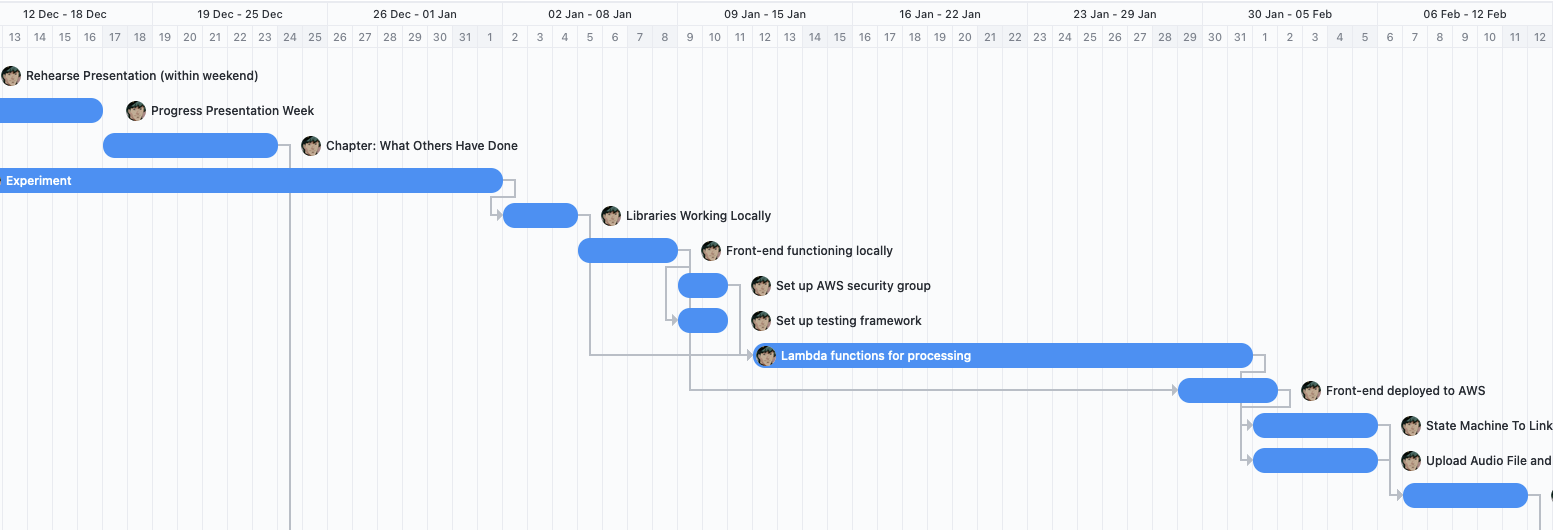
\includegraphics[width=\linewidth]{timeline1}
    \caption{Timeline: $Dec~12th~\rightarrow~Feb~12th$}\label{fig:timeline1}
    \endminipage\hfill
    \minipage{\textwidth}
    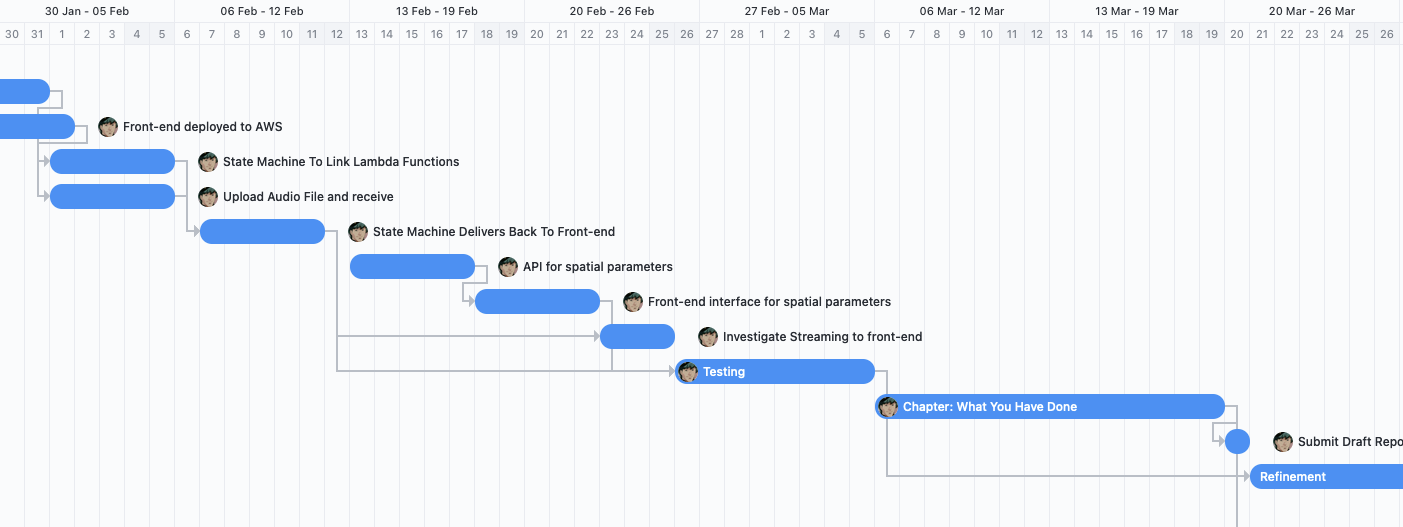
\includegraphics[width=\linewidth]{timeline2}
    \caption{Timeline: $Jan~30th~\rightarrow~Mar~26th$}\label{fig:timeline2}
    \endminipage\hfill
    \minipage{\textwidth}
    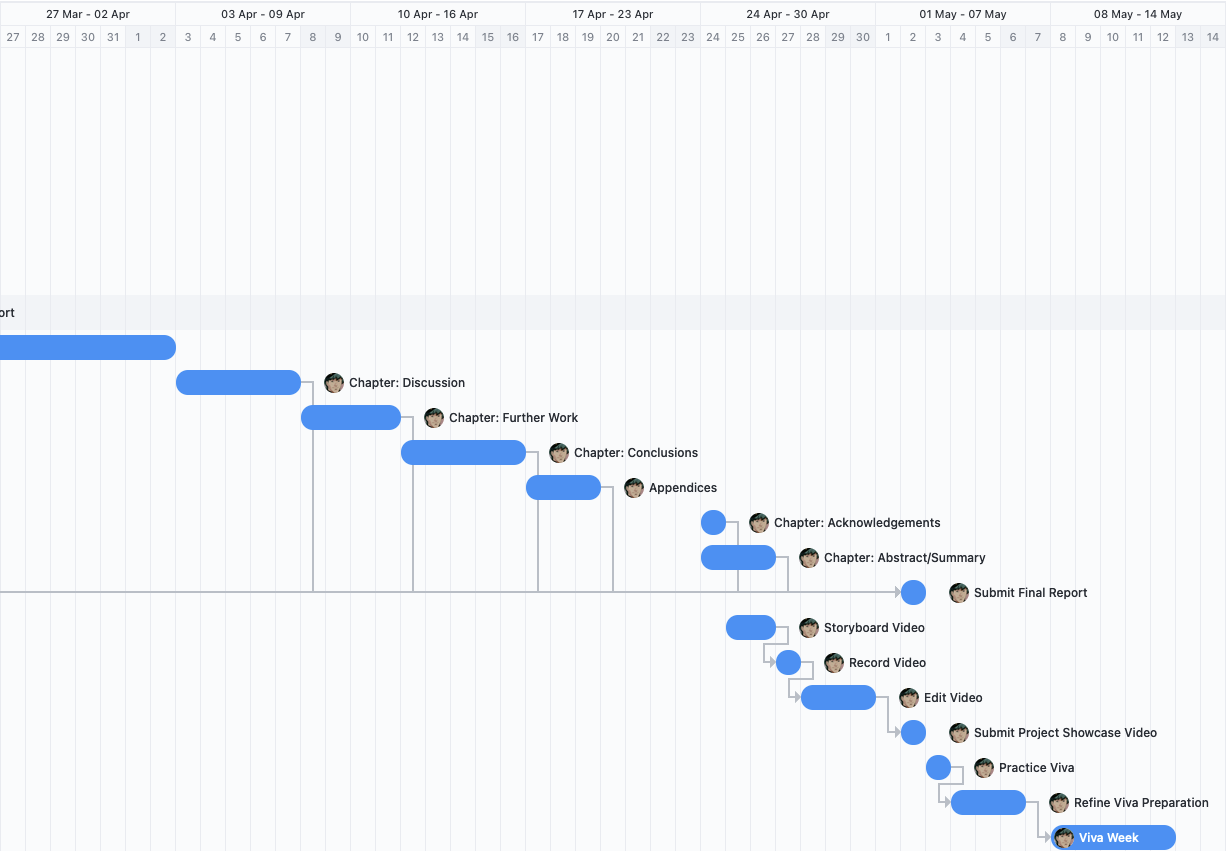
\includegraphics[width=\linewidth]{timeline3}
    \caption{Timeline: $Mar~27th~\rightarrow~May~14th$}\label{fig:timeline3}
    \endminipage
\end{figure}

\subsection{Resources}\label{subsec:resources}

This project intended to use minimal resources in its development.
As outlined in~\ref{sec:literature-review}, one of the many advantages of cloud computing is its flexibility and ease of resource management.
Given that the application would be hosted entirely in cloud environments, there would be no direct hardware costs associated with the project.
The costs that do apply will relate to the use of the~\gls{aws} platform.
These costs needed careful management, as explained in~\ref{subsec:business-risks}.

Other resources utilized included:

\begin{enumerate}
    \item Queen Mary library resources
    \item The project supervisor
    \item Knowledge sharing from colleagues at~\gls{sie}
    \item JetBrains’~\gls{ide} Suite
    \item Open-source audio-processing libraries.
    \item Online articles and tutorials
\end{enumerate}

\subsection{Methodology}\label{subsec:methodology}

\citet{murray-pm} notes that the \textquote{traditional} manner of software development follows a linear path from requirements, to design, to execution, to testing, and so on.
This method often results in inflexibility when it comes to software project execution.
This is because of its dependence on the full set of requirements being gathered before the development process begins.
Any issues with the requirements (incompleteness, inaccuracy) using this method are typically only found at the end of the process, instead of along the way through a cycle of development and feedback\footnote{\citep{murray-pm}}.
This project is of relatively small scope, and the number of shareholders are small on account of its proof-of-concept status.
As such, it serves to incorporate some, but not all, aspects of the `Agile'\footnote{\citep{beck2001agile}} development methodology into the process:

\begin{quotation}
    An Agile project starts with only the most high-level requirements.
    Sometimes these are referred to as “user stories.”
    Such a requirement might sound like, “A user will be able to buy a subscription to our product on a new e-commerce website.”
    There are no designs, no specifications.\footnote{\citep{murray-pm}}
\end{quotation}

While this project will not go so far as to remove the need for a design or specification altogether, the foundation for the project’s execution will rest on high-level user stories and identified functional requirements.
In addition, the project will require frequent testing as development progresses.
The intention, therefore, is to endeavour to implement a~\gls{cicd} pipeline to ensure any updates to the prototype can be tested and deployed in an online environment as it is being developed.

    \thispagestyle{plain}
\newpage
\section{Requirement Capture and Analysis}\label{sec:requirement-capture}

\normalsize

Primary functional requirements were well-defined.

\subsection{User Personas}

Persona of game developer:
want to experience what spatial audio can do therefore the project must be able
to take user input and render spatial audio based on that inputs as an MVP.

Persona of audio enthusiast:not necessarily a game Dev but someone who is interested in audio development who might like to try playing around with different spatial audio API without setting anything up locally.

Persona of the new user: Never experienced spatial audio, may not even know what it is.
Using the product and expecting to know more about what it means, not just what is available to developers.

Ultimately a rendering pipeline was needed in AWS. If the software can perform all audio processing in the cloud and deliver to frontend, that was MVP.

The project had other stretch goals: have a user interface that allows the user to input values; expand the functionality by specifying HRTF files and SOFA environment files; allow for real-time previewing.

These other goals were defined
by asking potential users + also experts in the field of audio processing in addition to the literature review.

Often more requirements came out in the form of user feedback.
Once people saw an early build, they came up with other `nice to have' features and requirements that went beyond the MVP\@.

MVP reqs:

Functional:
take user input.
separate and render audio in the cloud using HRTF profiles.
deliver output to frontend

Non-functional:
a UI to enter variables.
an elucidation of what spatial audio means: meet the intended stakeholder's requirements.
a 'good enough' delivery time - not so long that the user thinks it has failed

Stretch goal reqs:

Functional
- Preview spatial rendering of individual stems
- Real-time views of spatial audio
-- security - files are managed and secured to protect user info
- fast response time in rendering
- visual representation of the spatial audio rendering in 3d space
- allow user to upload and choose SOFA and BRIR files
- allow multiple types of audio file upload

Non functional
-- fully explains spatial audio and how it works
- a smooth looking ui - take it beyond basic to a potentially customer-facing product
- reliable - minimal bugs in the programming that result in failure for the end user.
- edge case handling



    \thispagestyle{plain}
\newpage
\section{Infrastructure \& Design}\label{sec:infrastructure-design}

\normalsize

Figure~\ref{fig:preliminary-design} details the initial design for the project's cloud architecture.
The diagram provides a high-level overview of the primary user journey,
and displays the~\gls{aws} products that were intended to fulfil this journey.
However, given that this project is executed using elements of the~\gls{agile} methodology,
this design was subject to change as development progressed.
This section aims to describe how the initial design evolved
to accommodate the changing system requirements of the project.

\begin{figure}[!htb]
    \minipage{\textwidth}
    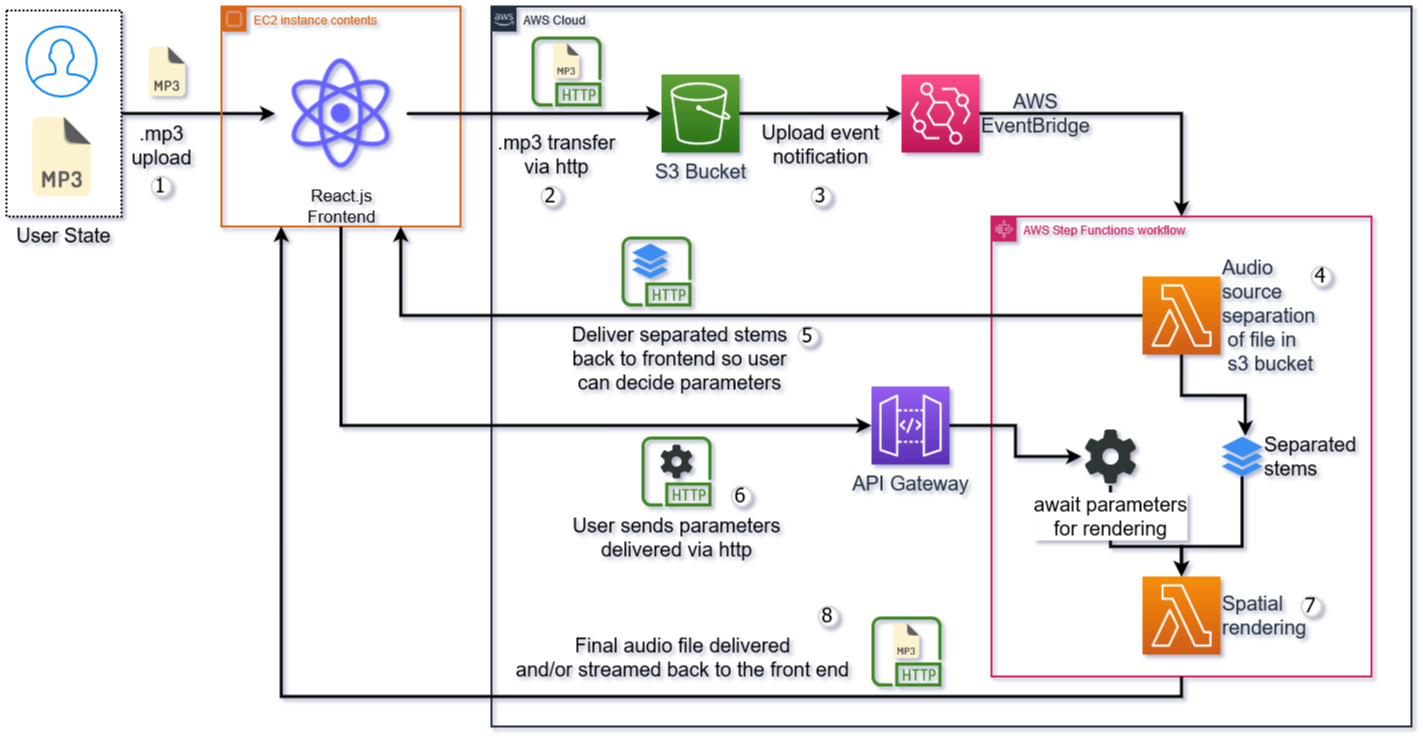
\includegraphics[width=\linewidth]{initial_architecture_diagram}
    \caption{Preliminary Design for Cloud Architecture}\label{fig:preliminary-design}
    \endminipage\hfill
\end{figure}

\subsection{Best Laid Plans}\label{subsec:best-laid-plans}

The product is designed for a wide range of users with varying knowledge of ~\gls{spatial_audio}.
In order to accommodate as many potential users as possible, a web-hosted~\gls{ui} is considered essential.
The user's primary mode of interaction with the service would be through a website
built using the~\gls{react} front-end library.
This library was chosen because of its ubiquity in modern web engineering, the depth of documentation available,
and existing familiarity with the framework.

The front-end was designed to make use of the~\gls{aws}~\gls{sdk} for~\gls{nodejs}.
This would allow the interface to initiate and interact with the audio processing pipeline hosted in~\gls{aws}.

Figure~\ref{fig:preliminary-design} displays the two~\gls{aws-lambda} functions
that would comprise the backbone of the audio processing pipeline.
Furthermore,
these~\gls{aws-lambda} functions would be coordinated and executed using the~\gls{aws-step-function} service.
This service was highly desired for this purpose
since the processing pipeline would follow a series of discrete steps that require input from the user.
\glspl{aws-step-function} would be able to accommodate this easily.

The entire service was initially intended
to be coordinated solely through the use of the internal messaging service:~\gls{aws-eventbridge}.
This service, in conjunction with~\gls{aws-api-gateway},
was intended to form most of the communication between the back and front ends of the application.

\subsection{Refinement}\label{subsec:refinement}

Problems with the initial designs were highlighted as the project progressed.

The first problems arose with the development of the~\gls{aws-lambda} functions that would be used to process the audio.
\gls{aws-lambda} functions
require a deployment package to be created
and then uploaded to~\gls{aws} in order for the function to have the resources it needs to run.
A fact that was not known previously is that
there is a limit of 50 MB on the size of the deployment packages that could be uploaded directly to~\gls{aws-lambda}.
Given that the 3D Tune-In Toolkit and the Spleeter source separation libraries have significant dependencies
that are more than 50 MB when zipped, a re-design needed to occur.

This issue was solved by making use of the~\gls{aws-ecr} service.
This service allows a developer to host and deploy~\glspl{container-image},
crucially, with a size limit of 75 GB allowed for each image uploaded to the registry.
Through the use of~\gls{docker} container images,
the code for the Lambda functions was bundled into deployment packages
that could be uploaded to an
\gls{aws-ecr} and then linked to a Lambda function
while staying well under the data limit offered by the container registry.
The Dockerfiles for the source separation and spatialisation lambda functions can be found in Appendix~\ref{subsec:lambda-function-dockerfiles}.
Note the installation of the AWS Lambda runtime environment for both Python in Listing~\ref{lst:source-sep-dockerfile} and C++ in Listing~\ref{lst:spatialisation-dockerfile}.

The next major revision to the architecture design came with the removal of the proposed~\gls{aws-api-gateway} interface.
Since the~\gls{aws-step-function} requires input from the user to execute,
the step function callback feature would be used to wait for an input message from the front end to the step function.
The most elegant solution for this problem was
to create a~\gls{aws-sqs} queue through which messages could be sent
and retrieved asynchronously without the risk of losing information through API communication failure.
This was implemented through the creation of a unique message queue per interaction with the product.
A unique identification key is created in the~\gls{react} interface, which is then used
to identify both the~\gls{aws-sqs} queue and the resources uploaded and retrieved from the relevant~\gls{s3} buckets.
This key is not the same as a session key
and would regenerate if the user refreshed the page to return to the start of the application.

With these changes, it became possible to define a final cloud architecture and workflow.

\subsection{Finalising the structure}\label{subsec:finalising-the-structure}

\begin{figure}[!htb]
    \minipage{\textwidth}
    \includesvg[width=\linewidth]{saas_architecture_2.0}
    \caption{Final cloud architecture diagram}\label{fig:final_design}
    \endminipage\hfill
\end{figure}

Figure~\ref{fig:final_design} depicts the final infrastructure design of the project.
The figure has been annotated with numbers to show the order in which data flows around the architecture.
In addition to the changes mentioned above, there are a few other notable changes that are evidenced in the figure.

\begin{itemize}
    \item The~\gls{aws-step-function} has been fleshed out with the discrete steps of the workflow orchestration.
    An Amazon States Language representation of the function can be found in Listing~\ref{lst:step-function-json}.
    \item There are three~\gls{s3} buckets to hold the artefacts from each stage of the process.
    \item The~\gls{react} frontend is now hosted in~\gls{amplify} instead of~\gls{ec2};
    allowing for the implementation of~\gls{cicd} each time a commit is pushed to a branch in GitHub.
\end{itemize}

\subsection{A fresh coat of paint}\label{subsec:a-fresh-coat-of-paint}

Early user testing of the product revealed
that elements of the front-end interface needed improving\footnote{Further information on the testing and feedback process can be found in Section~\ref{sec:testing-and-evaluation}}.
The initial interface was basic with minimal styling applied to the~\gls{react} interface.
See Figure~\ref{fig:early-fe} for a screenshot of the interface's early form.

\begin{figure}[!htb]
    \minipage{\textwidth}
    
\includegraphics[width=\linewidth]{early-ui}
    \caption{Early implementation of application frontend}\label{fig:early-fe}
    \endminipage\hfill
\end{figure}

After the~\gls{mvp} was achieved, there was some additional capacity available to improve the frontend.

\begin{itemize}
    \item The project was adapted to use tools provided by~\gls{mui},
    a~\gls{react} component library\footnote{https://mui.com/core/},
    in order to better structure the project and improve the aesthetic feel.
    See Figure~\ref{fig:ui-splash} for the improved welcome screen for the application.
    \item A slideshow was developed using the component library that explained the theory behind spatial audio in an easy-to-understand manner and explains what the product aims to do (Figure~\ref{fig:ui-slideshow}).
    \item The music file upload stage of the application was redesigned using~\gls{mui} and turned into a three-step process using the `Stepper' component (Figure~\ref{fig:ui-uploader}).
    \item The `Spinner' component is used to help decorate the process of waiting for the stems to be separated out (Figure~\ref{fig:ui-spinner}).
\end{itemize}

\begin{figure}[!htb]
    \minipage{\textwidth}
    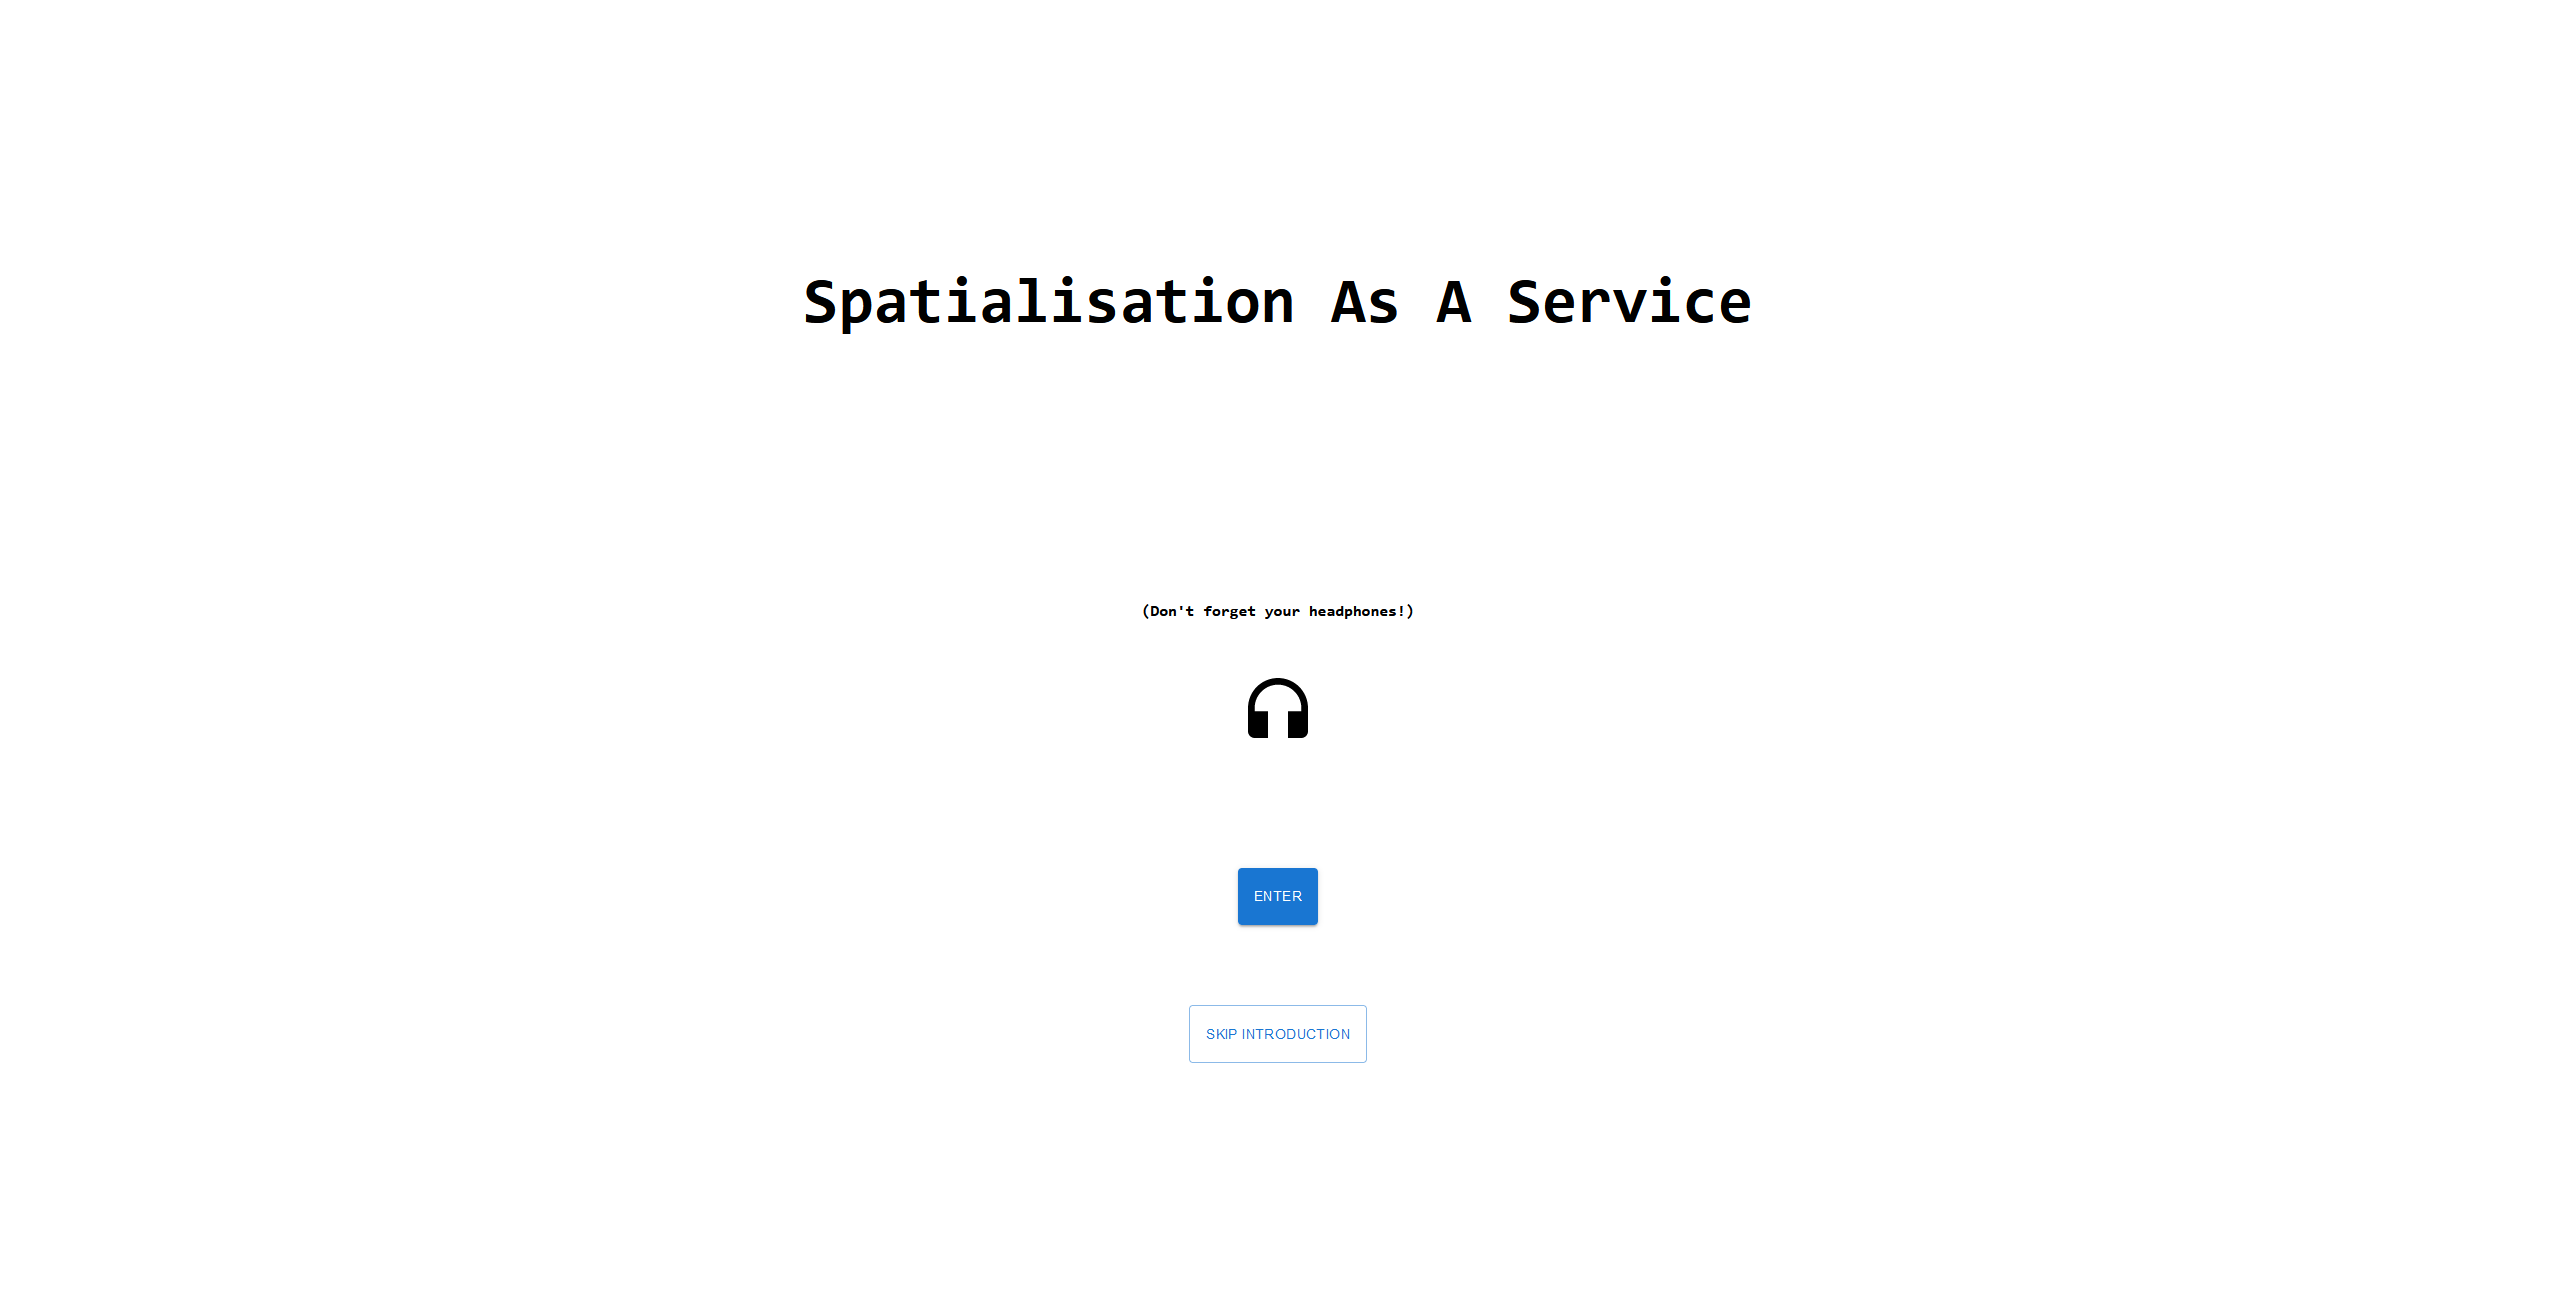
\includegraphics[width=\linewidth]{ui-splash}
    \caption{Refined splash screen that greets the user}\label{fig:ui-splash}
    \endminipage\hfill
\end{figure}

\begin{figure}[!htb]
    \minipage{\textwidth}
    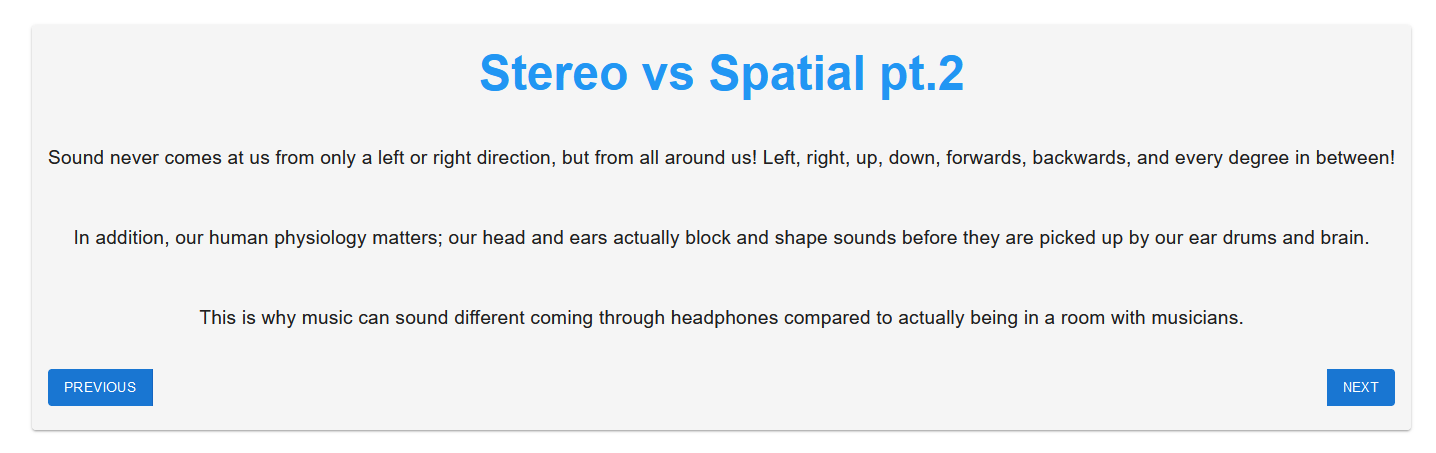
\includegraphics[width=\linewidth]{ui-slideshow}
    \caption{One of the slides from the introductory explanation of the project}\label{fig:ui-slideshow}
    \endminipage\hfill
\end{figure}

\begin{figure}[!htb]
    \minipage{\textwidth}
    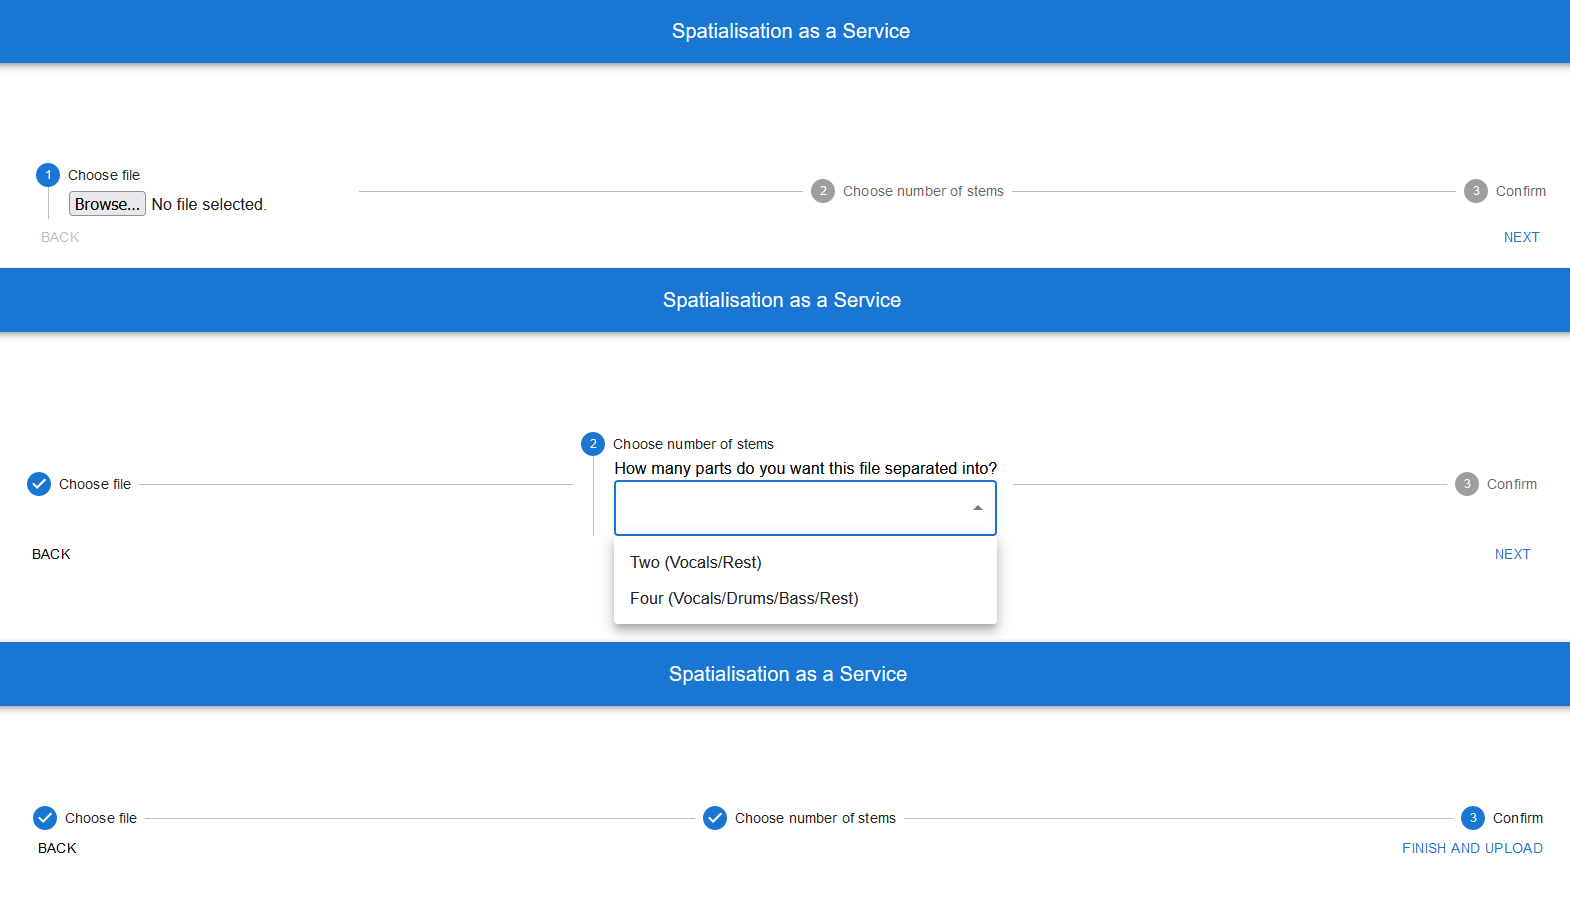
\includegraphics[width=\linewidth]{ui-uploader}
    \caption{Audio upload stage remodelled using the~\gls{mui} Stepper component}\label{fig:ui-uploader}
    \endminipage\hfill
\end{figure}

\begin{figure}[!htb]
    \minipage{\textwidth}
    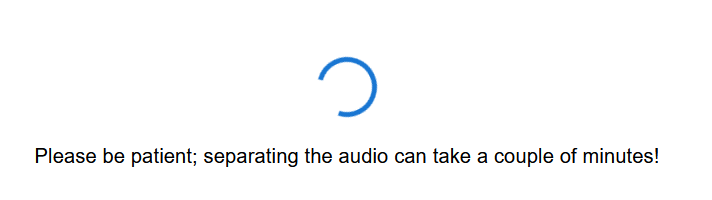
\includegraphics[width=\linewidth]{ui-spinner}
    \caption{\gls{mui} Spinner and message displayed while audio stems are separated}\label{fig:ui-spinner}
    \endminipage
\end{figure}

\subsection{No spatialisation without representation}\label{subsec:no-spatialisation-without-representation}
An important piece of feedback on early demos of the product was that there was not enough visual or audio feedback on the user's input of the spatial parameters.
As a result of this,
the most significant redesign of the product allowed the user
to experience and preview the effects of their input
instead of being forced to wait for the final product to render and be delivered to the frontend.
Using React Three Fiber, a~\gls{react} renderer for~\gls{threejs}\footnote{\citep{dirksen2023learn}},
a 3D model represents the positioning of the audio stems in the virtual spatial field
that the application eventually renders.
The input fields for each stem's spatial positions are now overlaid on top of the model.
Previously only lists of sliders were shown for each stem,
but the final version lets
the user see and hear what changes are being made in real-time as the stems are being played back.
Figures~\ref{fig:ui-3d-1},~\ref{fig:ui-3d-2},
and~\ref{fig:ui-3d-3} demonstrate how the 3D model displays the user's input on screen.
The user is able
to rotate and zoom in and out of the model
to see where the stems are positioned in relation to the listening position at the origin of the model.
In addition, instead of the stems being played separately as before, the stems synchronise to each other,
and the user can mute or `solo' each stem as they wish.
This functionality is similar to that found in modern Digital Audio Workstations.
The Howler.js library,
which is used for audio playback, allows the accessing of the spatial audio module in the Web Audio API\@.
Because of this, the user can preview the audible position of each stem while they are playing in the application.
However,
the quality of this preview is not as high-quality as the final rendered output that is created using the 3D-TuneIn API;
this justifies the retention of the option to render the audio using the workflow hosted in~\gls{aws-lambda}.

\begin{figure}[!htb]
    \minipage{\textwidth}
    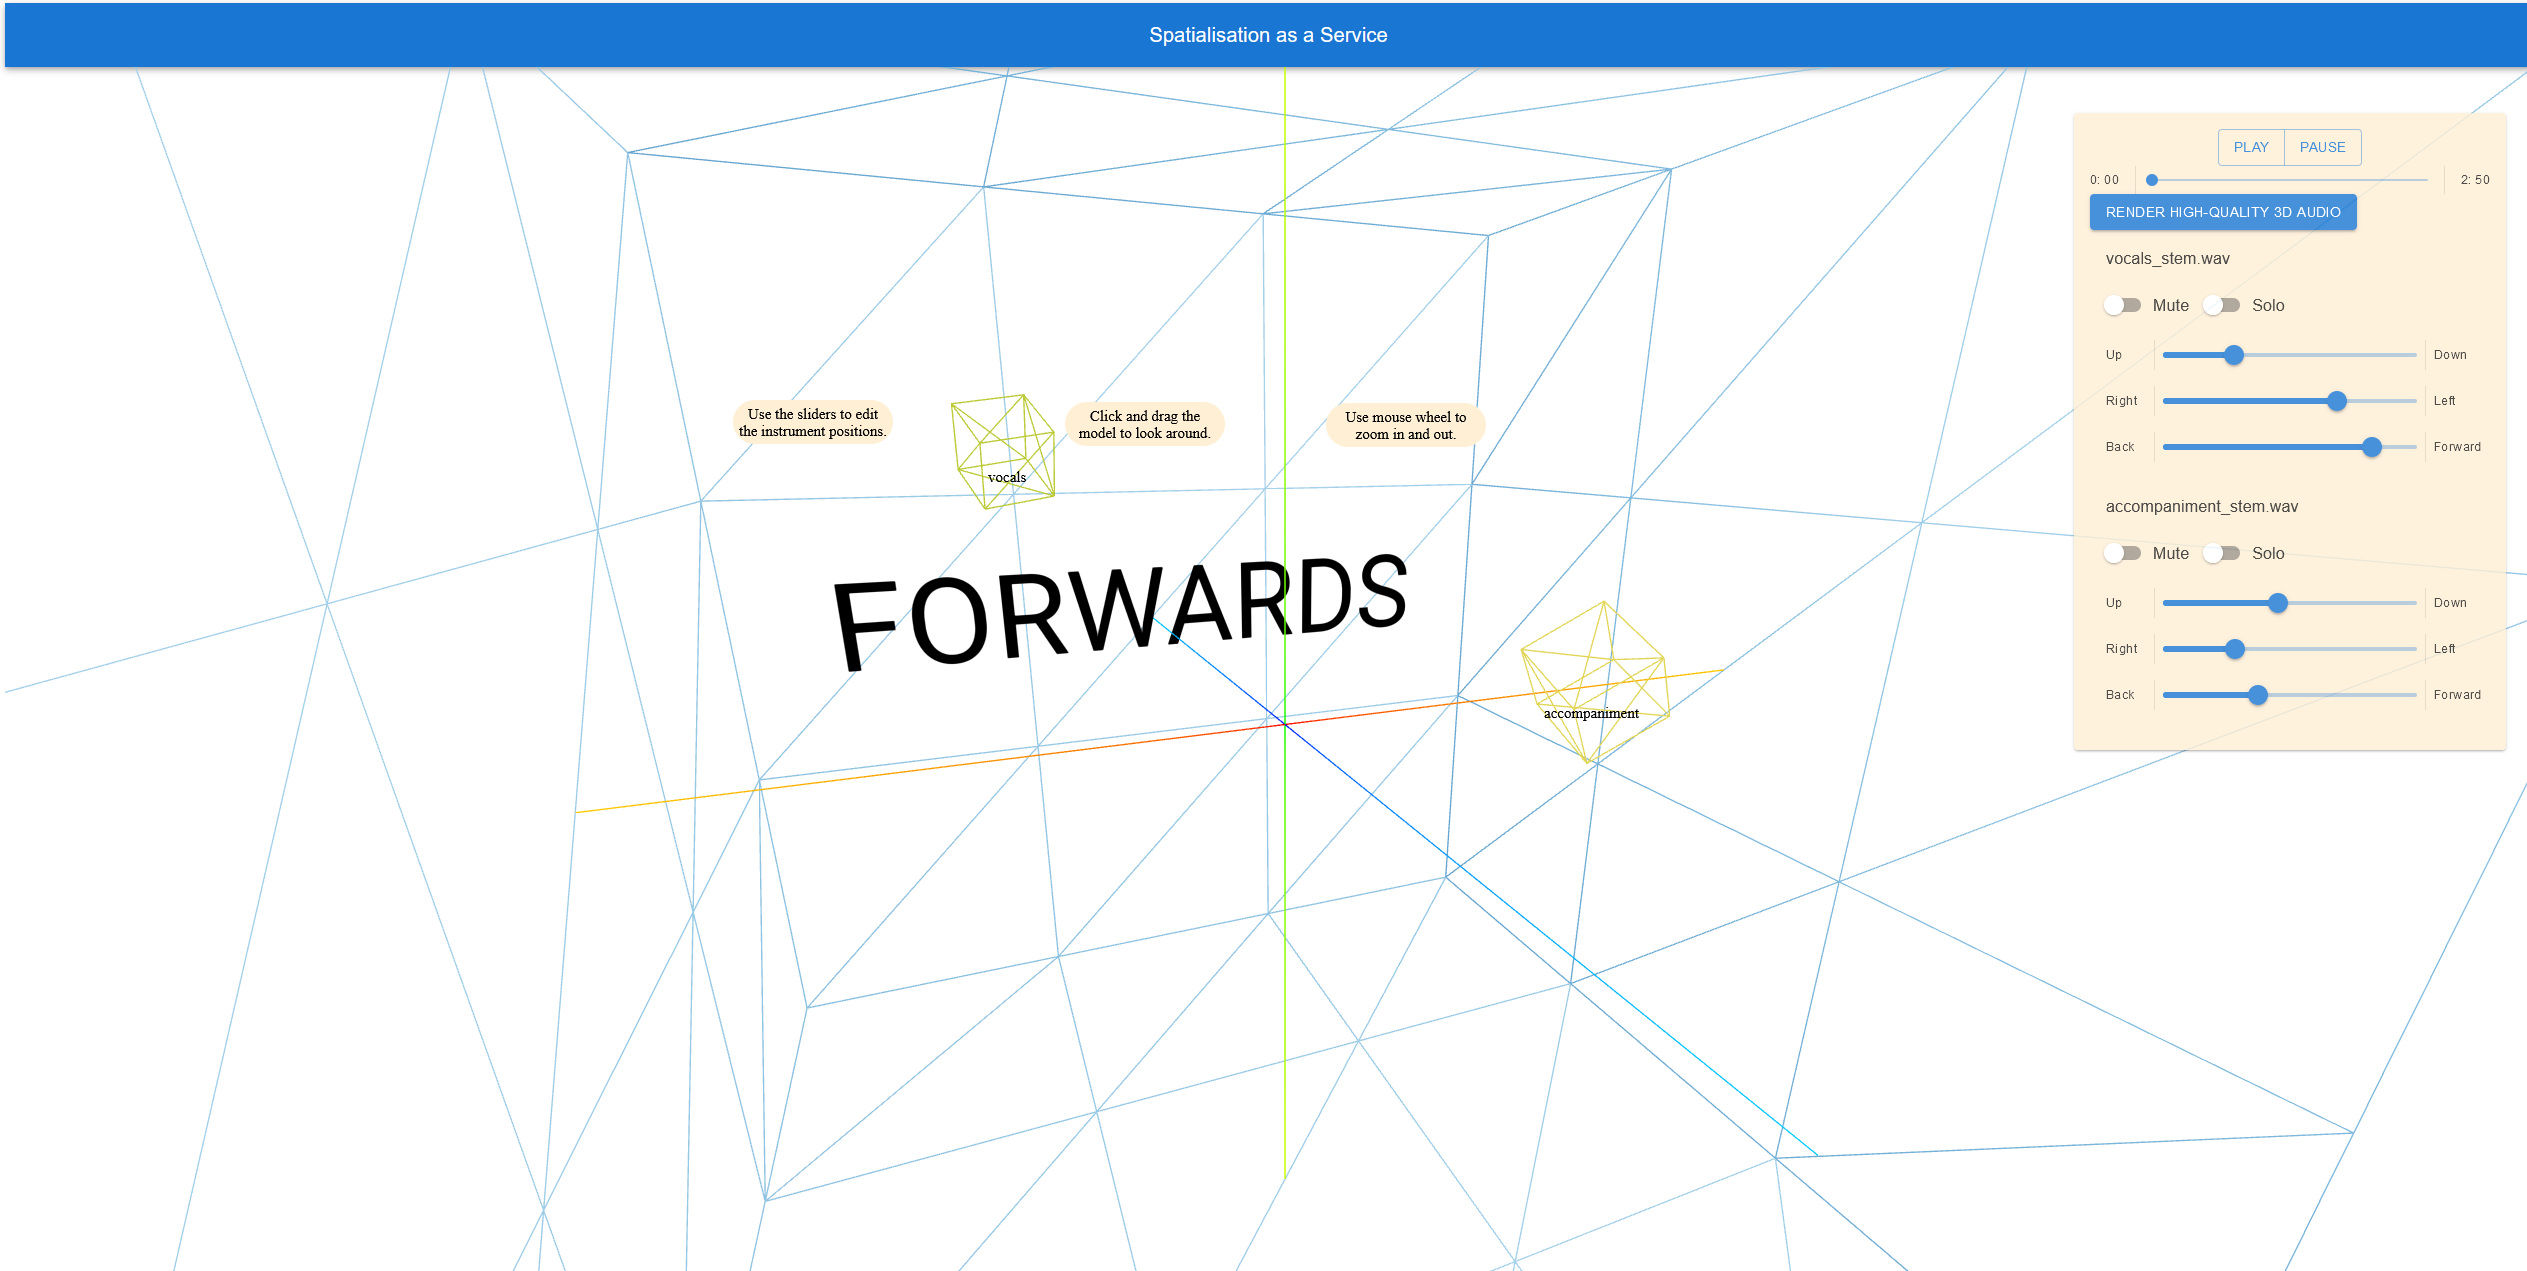
\includegraphics[width=\linewidth]{ui-3d-1}
    \caption{Perspective 1 of the 3D model interface}\label{fig:ui-3d-1}
    \endminipage
\end{figure}

\begin{figure}[!htb]
    \minipage{\textwidth}
    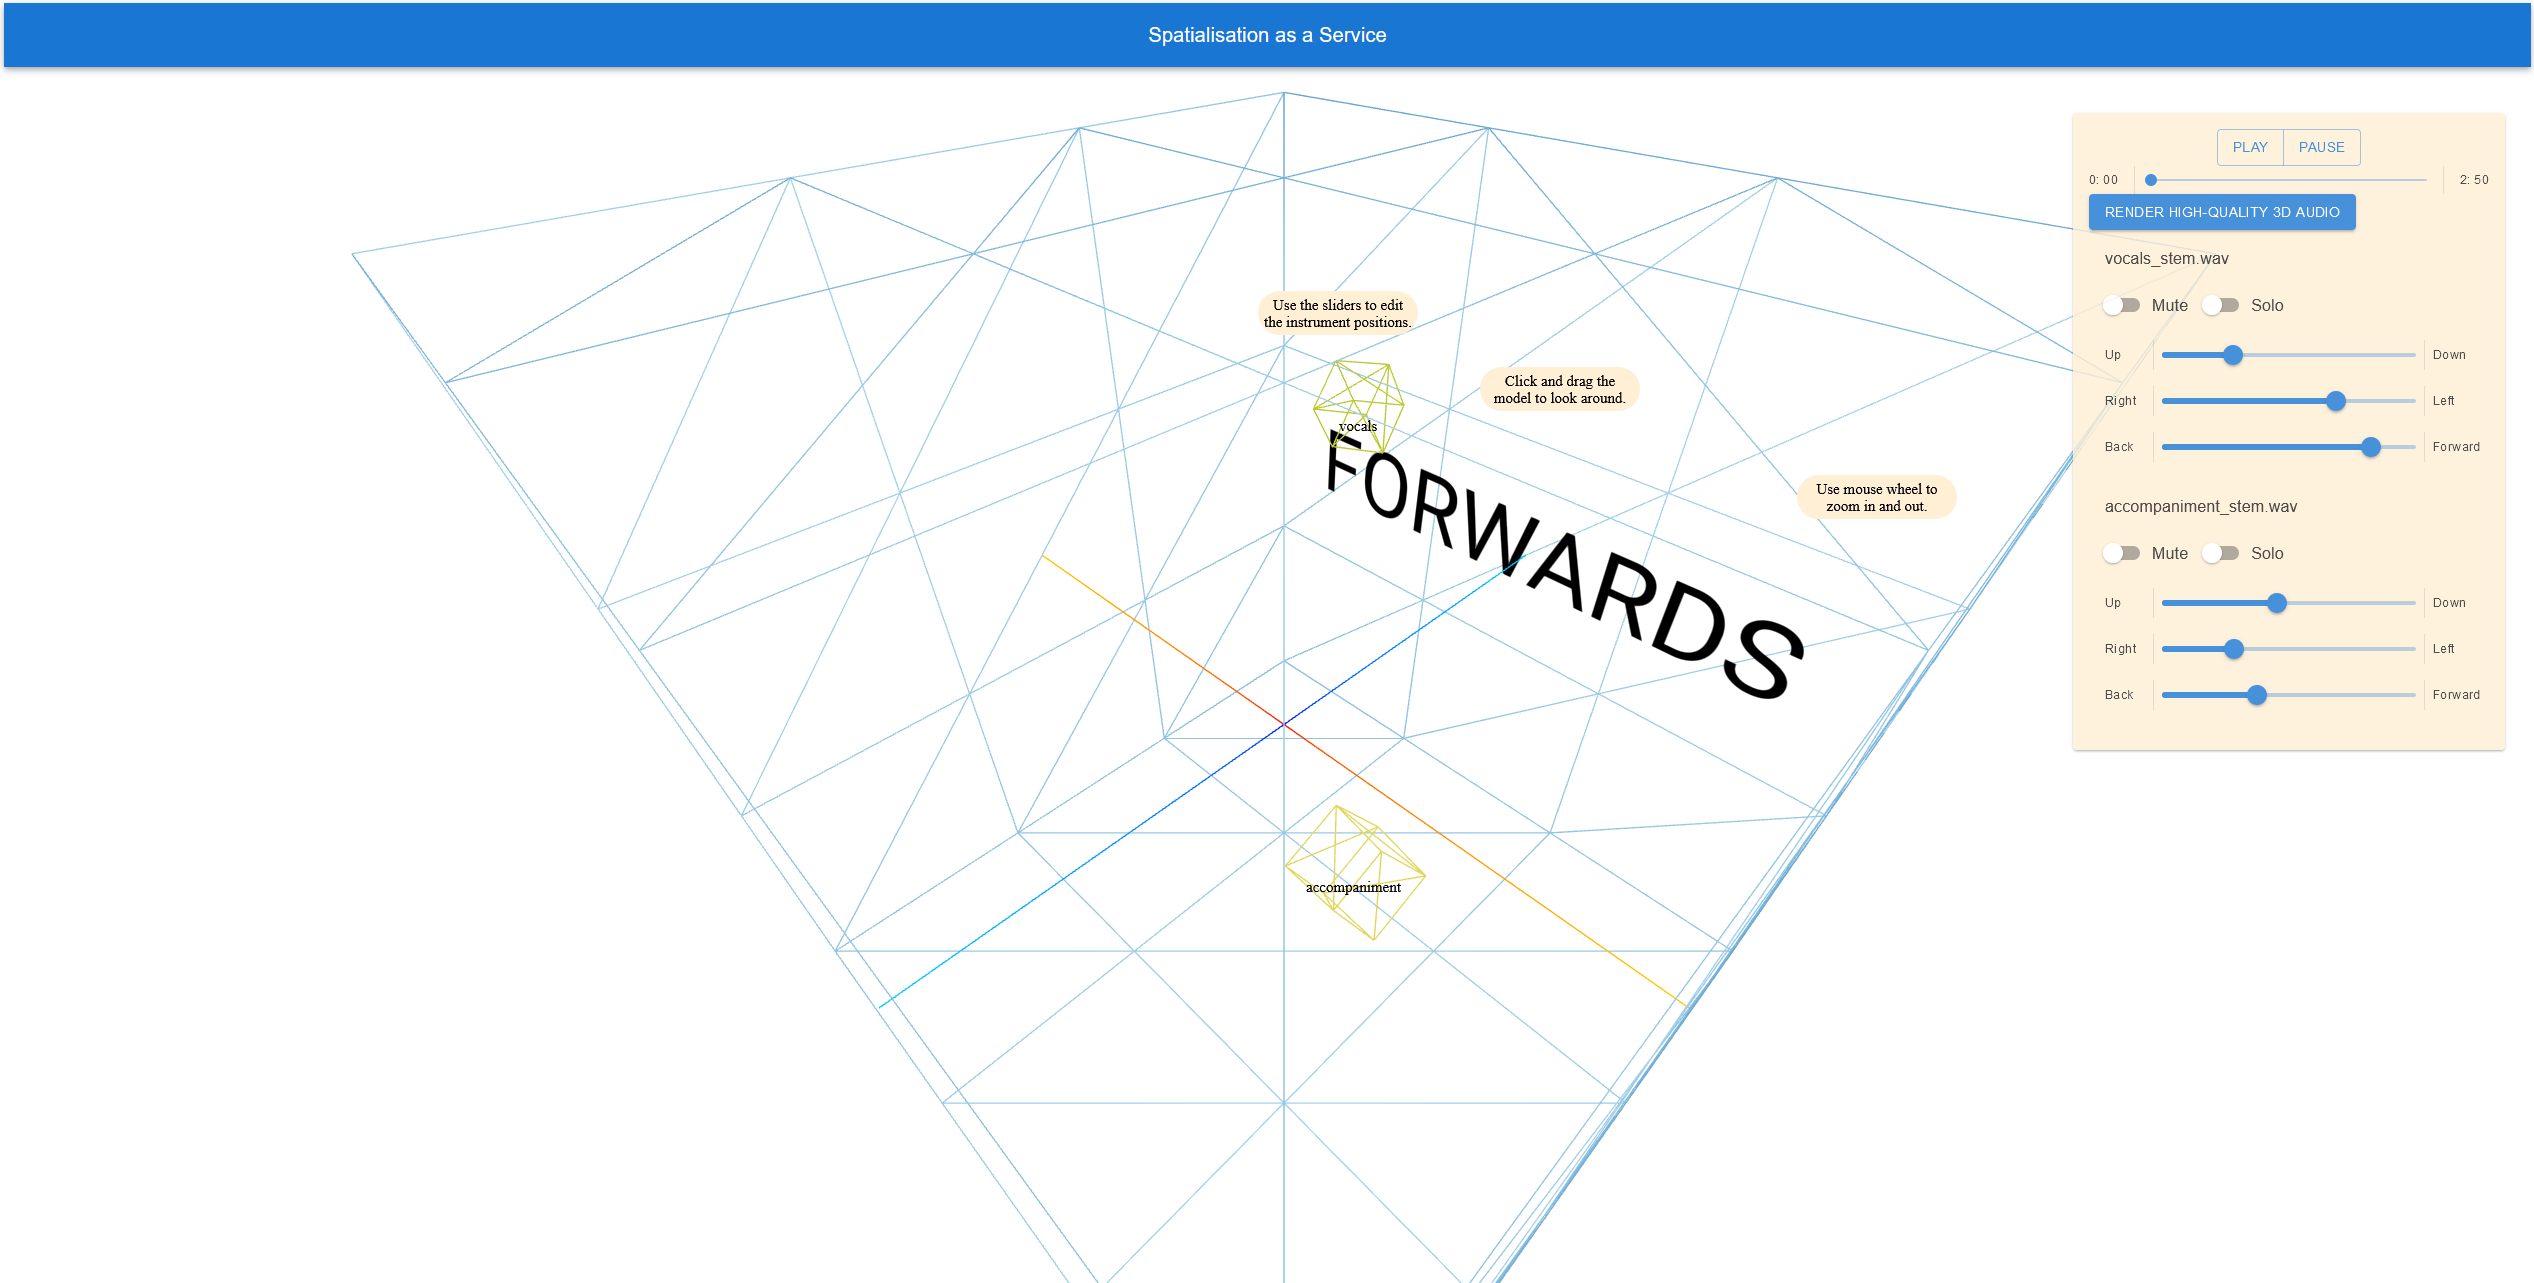
\includegraphics[width=\linewidth]{ui-3d-2}
    \caption{Perspective 2 of the 3D model interface}\label{fig:ui-3d-2}
    \endminipage
\end{figure}

\begin{figure}[!htb]
    \minipage{\textwidth}
    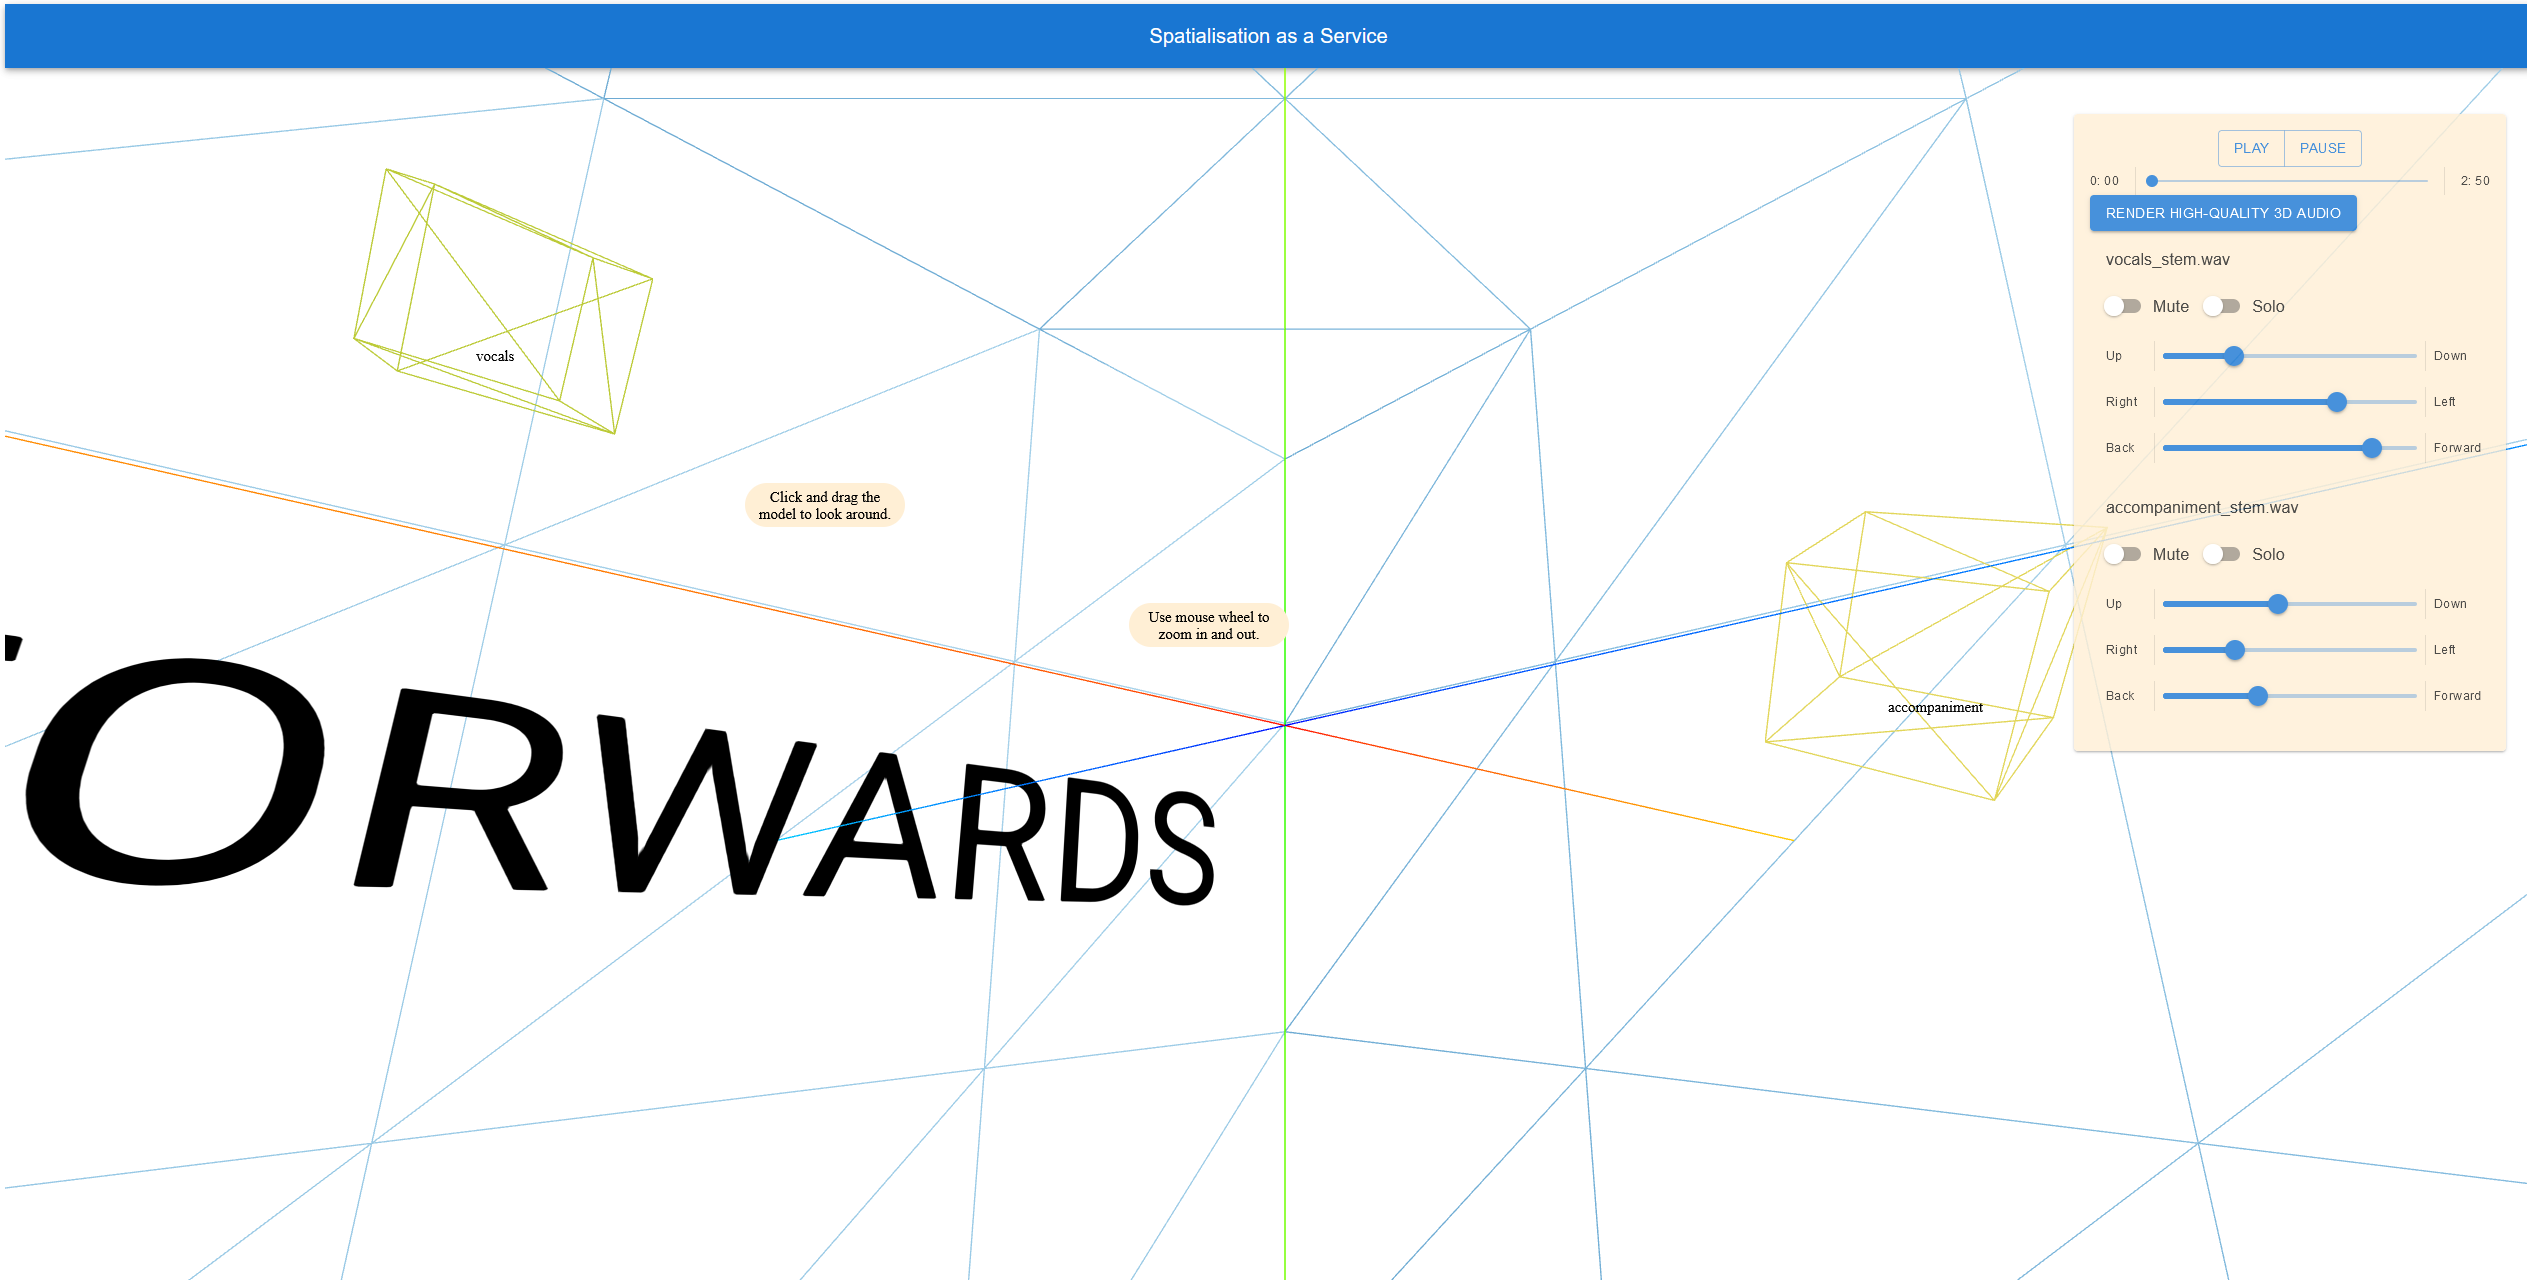
\includegraphics[width=\linewidth]{ui-3d-3}
    \caption{Perspective 3 of the 3D model interface}\label{fig:ui-3d-3}
    \endminipage
\end{figure}
    \thispagestyle{plain}
\newpage
\section{Implementation}\label{sec:implementation}

\normalsize

\subsection{Start Small, Aim Big}\label{subsec:start-small-aim-big}

Section~\ref{sec:requirement-capture} details how the~\gls{mvp} for the project was formulated from the system requirements.
Given the complexity of the project,
it was advantageous to break down the elements of the system into smaller,
more atomic tasks that each worked towards a requirement.
Some of these discrete tasks can be seen in Figures~\ref{fig:timeline1},~\ref{fig:timeline2}, and ~\ref{fig:timeline1}.
By breaking down tasks in this way,
it was
easier to make incremental progress
rather than be overwhelmed by the complexity of the overall project.
The development strategy was to reach the~\gls{mvp}, overcome obstacles along the way,
and then refine further based on feedback from users.
Since much of the~\gls{mvp} was based on the system's functionality,
there was not a focus on the user experience at the outset of the project;
a flashy front-end was low on the initial list of priorities.

\subsection{Continuous Integration / Continuous Deployment}\label{subsec:continuous-integration-continuous-deployment}

As seen in Figure~\ref{fig:final_design}, the project is made up of a number of discrete modules that link together.
Furthermore, the~\gls{react} front-end comprises a number of interlinked components.
The development process saw the steady addition and refinement of modules and components to reach the final version.
However, given the interconnectedness of the system,
it was important to ensure that changes to the project did not affect older modules or components.
A common method of avoiding these breaking changes in industry is
to use~\gls{cicd}~\citep{duvall2007continuous, miller-ci}.

A~\gls{cicd} pipeline was set up using a combination of the Git version control software and~\gls{amplify}.
Each time a commit was pushed to the repository,
a build of the project was executed and then immediately deployed to an online environment.
As a part of the build,
a suite of~\gls{playwright}\footnote{In addition to end-to-end testing, an update to~\gls{playwright}'s feature set allowed for the testing of individual~\gls{react} components that could be mounted and tested independantly from one another.} automated tests was run
to ensure that the functionality previously established had not been compromised by the new commit.
Using this workflow, it was easy to identify issues when they occurred.

\begin{figure}[!htb]
    \minipage{\textwidth}
    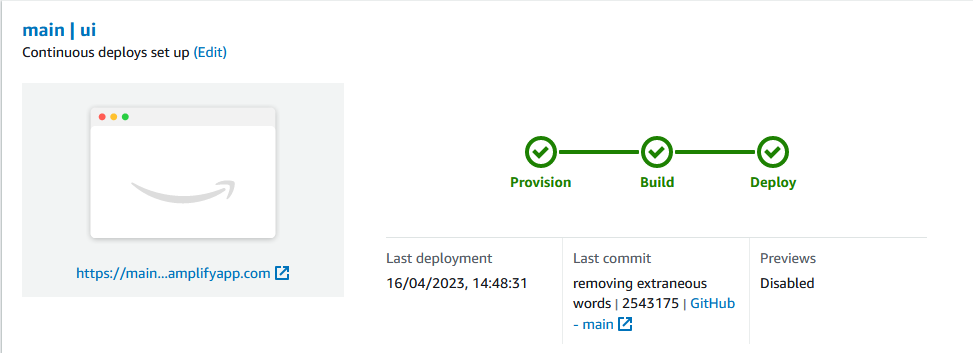
\includegraphics[width=\linewidth]{amplify}
    \caption{A screenshot of the~\gls{amplify} dashboard showing the successful provisioning, building, and deployment of a branch from the project repository}\label{fig:amplify}
    \endminipage
\end{figure}

This workflow enabled the use of parallel builds, which were utilised when the time came for user testing.
~\gls{amplify} is able to create a separate build and deployment for different branches of a GitHub repository
(Figure~\ref{fig:amplify}).
A version of the project was deployed for user testing alongside the main development branch.
This prevented new additions to the development branch disrupting the user testing version and deployment.

\subsection{Trials and Tribulations}\label{subsec:trials-and-tribulations}
During development of the project, a number of challenges and problems were encountered.
The project required the learning of a range of new pieces of software,
such as the~\gls{aws}~\gls{sdk} and~\gls{docker}.
This meant
that most delays to the project were due to insufficient knowledge
that needed to be corrected through reading documentation and examples that are hosted online.
However, some issues were far more significant and will be detailed below.

\subsubsection{The Recursion Incident}\label{subsubsec:recursion-incident}

The major incident of the project stemmed from the accidental over-allocation of~\gls{aws} resources.
A previous version of the orchestrating~\gls{aws-step-function} was triggered
when a file was uploaded to a~\gls{s3} bucket.
The~\gls{aws-step-function} then triggered the source-separation~\gls{aws-lambda} function
which contained a bug where the output of the function was deposited to the originating s3 bucket.
The depositing of the resultant stems then triggered another~\gls{aws-step-function} for each stem
deposited because of the aforementioned triggering rule.
Since the output of the source separation function was (at this point) two stems,
there was a recursive re-triggering of the step function
which increased the number of invocations and stored output stems at a quadratic rate.
Making matters worse,
this error was not noticed for at least a period of twenty minutes\footnote{As this author was on the London Underground!}.
This recursive invocation, despite triggering a number of Lambda throttles,
resulted in a large bill from~\gls{aws} since there is a charge per invocation (Figure~\ref{fig:incident-invocations}).
In addition,
the size of the files created was 1.3TB
and there were additional charges from~\gls{s3} due to the amount of data created and stored via~\gls{api} calls
(Figure~\ref{fig:incident-storage}).

\begin{figure}[!h]
    \centering
    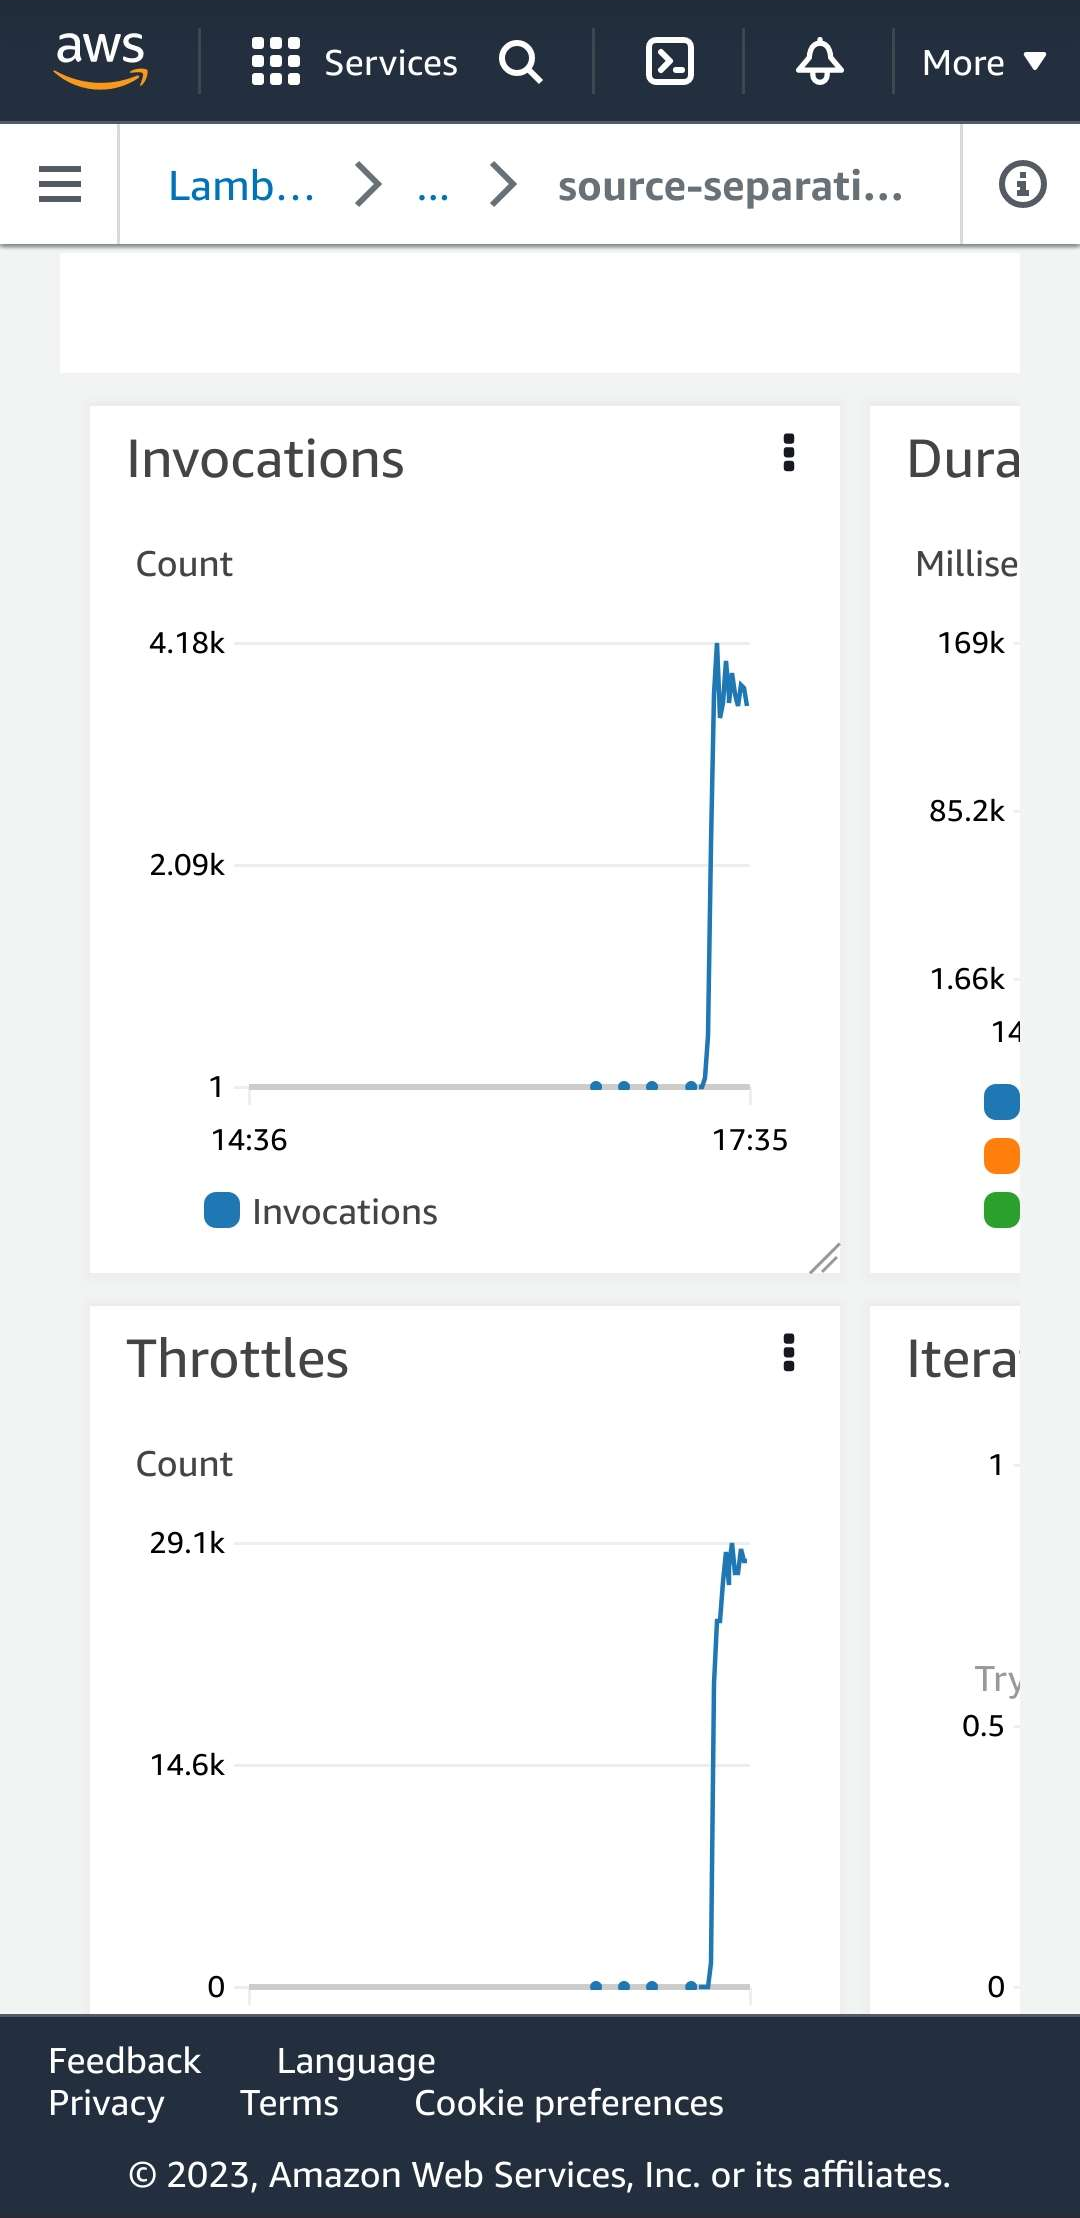
\includegraphics[height=20cm, keepaspectratio]{incident-invocations}
    \caption{A graph of the number of invocations and throttle over the time of the incident}\label{fig:incident-invocations}
\end{figure}

\begin{figure}[!h]
    \centering
    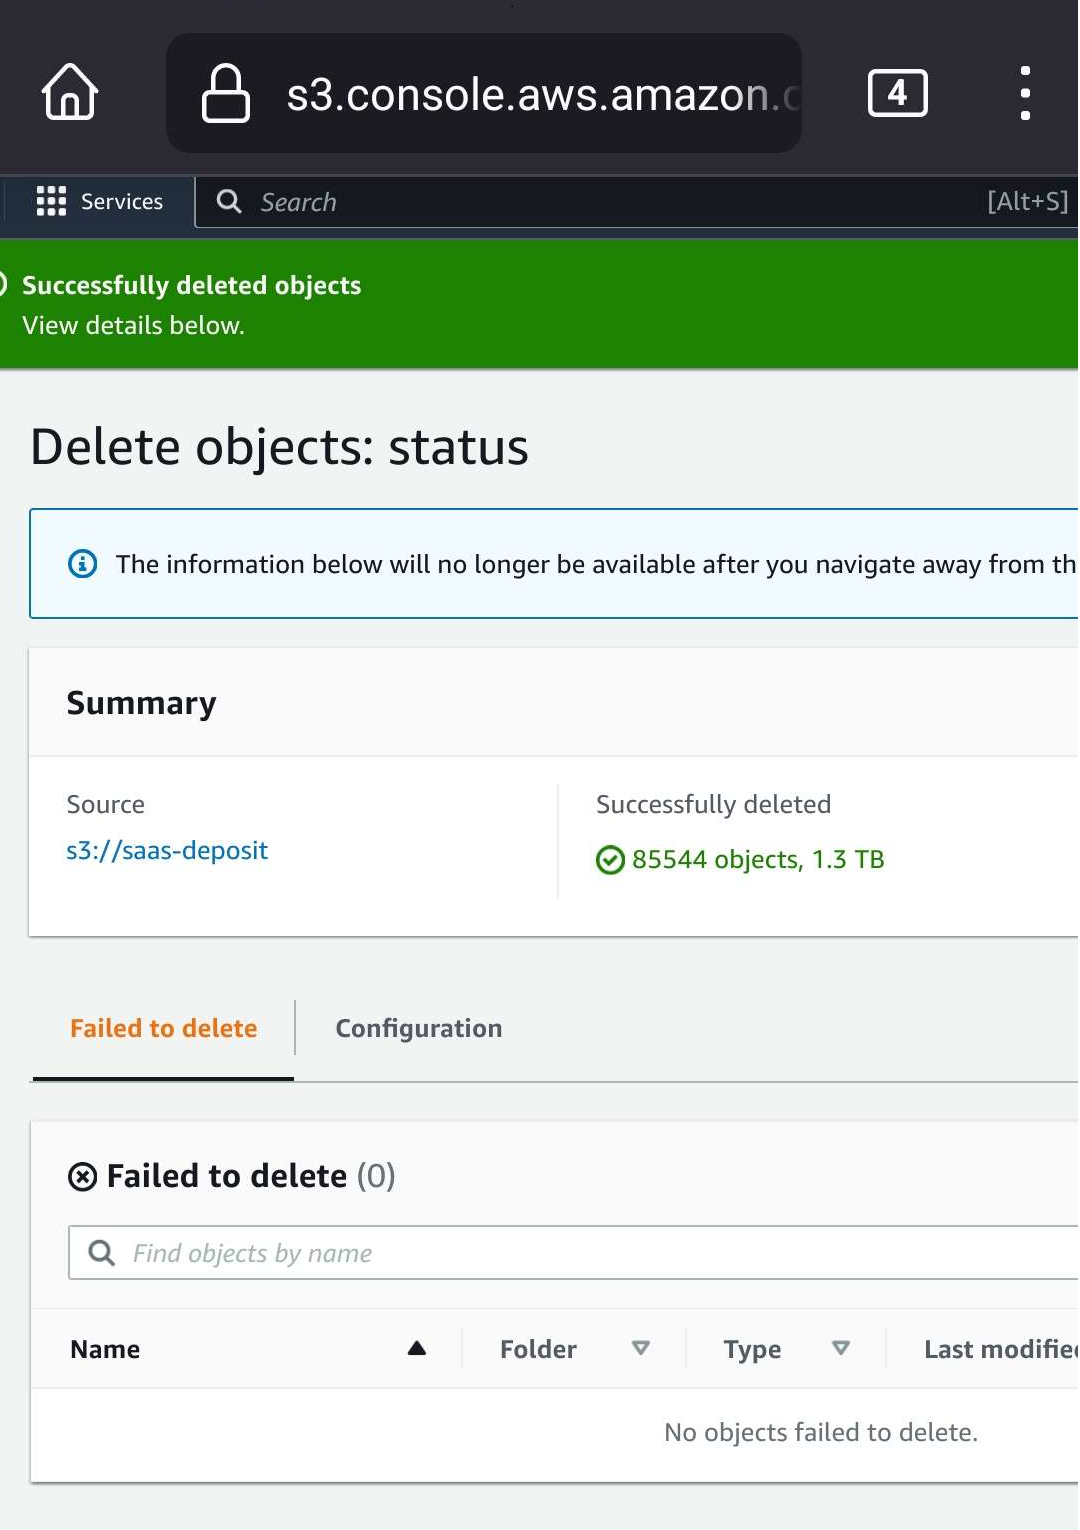
\includegraphics[height=20cm, keepaspectratio]{incident-storage}
    \caption{The size of the total objects deleted from the~\gls{s3}} bucket\label{fig:incident-storage}
\end{figure}

Thankfully~\gls{aws} customer service was understanding and forgave the charges
incurred on that day since it was a mistake.
However,
the situation stands as evidence
that developing for public cloud services poses a tangible risk as identified in~\ref{subsec:business-risks}.
The breakdown of the usage costs on the day of the incident can be found in Figures~\ref{fig:cost-graph} and~\ref{fig:cost-breakdown}.

\begin{figure}[!htb]
    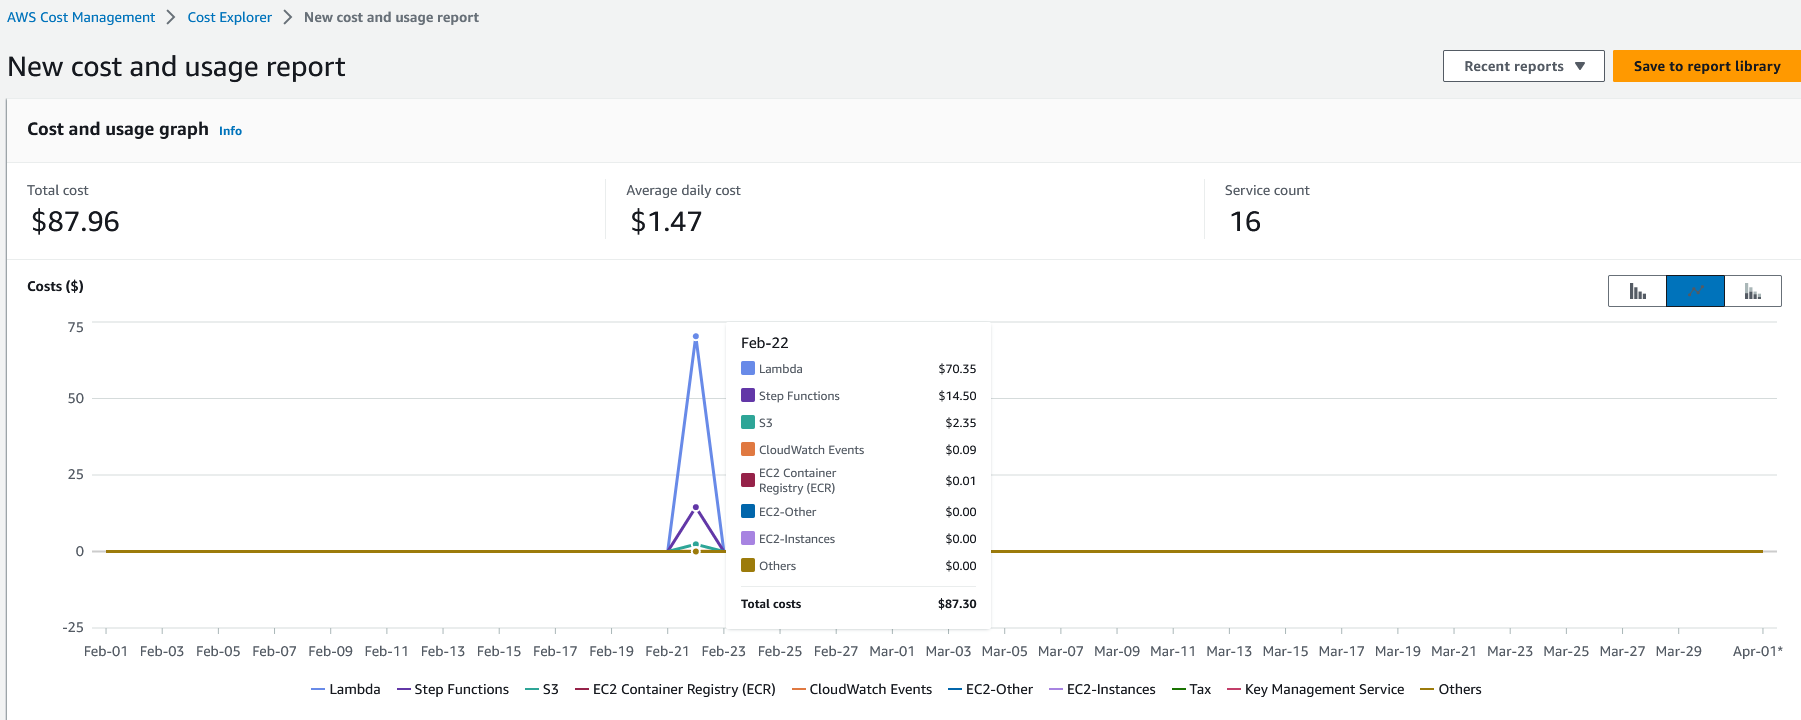
\includegraphics[width=\linewidth]{cost-graph}
    \caption{A graph showing the distribution of accidental charges in a wider billing period}\label{fig:cost-graph}
\end{figure}

\begin{figure}[!h]
    \centering
    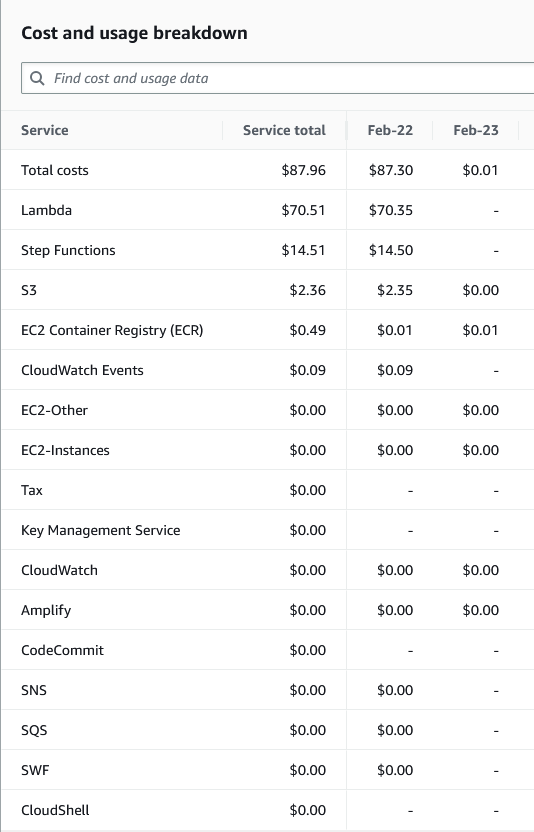
\includegraphics[height=20cm, keepaspectratio]{cost-breakdown}
    \caption{A granular breakdown of AWS costs on the day of the incident compared to the total costs for the duration of development. Fields with the value of \$0.00 mean that the service is in use, but hasn't used enough to incur charges}\label{fig:cost-breakdown}
\end{figure}




-- after results of user testing I needed to refine the product.
Front end component was missing - much more time needed to be put into react.js, MUI and playwrights test writing to accommodate new react components at the unit test level
-- not so much feature creep than lack of time for proposed complexity - desired features required much more learning than previously thought, especially in docker builds and cmake structures
-- local builds proved difficult for Dev purposes, often had to wait for docker images to be built and uploaded and changes to react to be built and deployed using amplify, lots of dev time eaten up waiting

— Code refactor and documentation towards the end of the project to maximise readability
    \thispagestyle{plain}
\newpage
\section{Testing and Evaluation}\label{sec:testing-and-evaluation}

\normalsize

Testing was a continuous process. Given the nature of the cloud environment things needed to be deployed in an environment so they could be tested.

This is why CI/CD was used.
Commits and pushes to AWS
triggered redeployments and the ability
to test changes in a cloud environment quickly in addition to running regression tests each time.

Manual testing was required to ensure functionality was there but user testing was also used.
A form and a link to an early build of the product were sent out and responses collected. These responses helped assess the effectiveness of the products functionality and guide future development processes.

Product was a success in not only delivering intended functionality but also extending it beyond the static spatial rendering but also preview the spatial audio in a real-time environment.
Front end was far more in depth after refinement
    %! Author = callum
%! Date = 25/03/2023

% Preamble
\documentclass[11pt]{article}

% Packages
\usepackage{amsmath}

% Document
\begin{document}



\end{document}
    \thispagestyle{plain}
\newpage
\section{Further Work}\label{sec:further-work}

\normalsize

\subsection{Cold Starts}\label{subsec:cold-starts}

When one is using the service, the least performant step is the stem separation stage.
Since the source separation lambda function uses TensorFlow,
its long initialisation time causes this stage of the process
to run slowly as most of the wait time is dedicated to the initialisation of TensorFlow,
rather than the processing time itself.
This \textit{cold-start}
time between initialisation and runtime is something
that would be targeted for improvement in future versions of the project.
Since this is the most impactful performance issue of the product, this would be the first priority.

\subsection{Custom SOFA Files for HRTF and BRIR}\label{subsec:custom-hrtf-and-hrir-files}

One of the major benefits
of using the 3D Tune-In Toolkit over the spatial module in the Web Audio API is that it allows the use of different~\gls{hrtf} profiles for spatialisation.
The toolkit is customizable and offers a greater fidelity of spatialisation over Web Audio.
A further improvement to the product would be
to allow the use of user-specified SOFA files for the rendering of spatial audio.
SOFA files contain the data necessary to produce the~\gls{hrtf} and~\gls{brir} necessary for the service's rendering of the audio.
The ability
for the user to upload their own files would greatly improve the depth of customization the product can offer.

\subsection{Further UI Improvements}\label{subsec:ui-improvements}

The remodelling of the initial user interface as described in~\ref{subsec:a-fresh-coat-of-paint} was extensive,
however, it is clear there is still room for improvement.
Some ideas for further~\gls{ui} and~\gls{ux} improvements are:
\begin{itemize}
    \item Add a loading bar to the source separation stage so that the user has an indication of when it will finish.
    \item Make the 3D model change to match different~\gls{brir} if a custom SOFA file is uploaded for rendering.
    \item Change the real-time preview of the spatialisation to use the 3D Tune-In Toolkit to increase the quality and accuracy of the preview.
    \item Make the~\gls{ui} more detailed and precise; take it beyond a demonstration and make it more production-ready.
\end{itemize}

\subsection{Functional Improvements}\label{subsec:functional-improvements}

More generally the product could improve the following aspects of its functionality:

\begin{itemize}
    \item Speed up the overall time it takes to separate the files and render the final audio
    \item Provide more options for source separation; currently the service is only set up to separate music files with vocals and further support could be provided for instrumental tracks through training the TensorFlow model stored in the~\gls{aws-lambda} function.
    \item Improve the security of the project by tightening the policies attached to the~\gls{s3} buckets holding the data, despite the lifecycle rules put in place.
\end{itemize}
    \thispagestyle{plain}
\newpage
\section{Discussion \& Conclusions}\label{sec:discussion-conclusions}

\normalsize

Success based on the initial criteria of the project. Met the core functional requirements and succeeded in creating a cloud-based service that is genuinely unique and allows easy access to trialling high-quality spatial audio to anyone with a browser and a music file.

Additionally, user feedback was very good - most were impressed with the core product despite having reservations about the user interface and its ability to convey information and instructions to the user.

However, the major issue with the project was in its inaccurate user requirements that needed redefining in the face of feedback. Initially was only concerned with the functionality for MVP. However didn't not fully consider the fact that it was real people using the project who may not initially understand what the software did. User experience was far more important than initially thought to user satisfaction. To the extent that some users did not understand the idea of spatial audio and confused the product with stereo music making software.

Given this, I did a good job of pivoting and, once the core functionality of cloud architecture was finished, spent a lot more time refining the user experience. This resulted in: a slideshow explaining the process, a much more refined ui, and even a live mockup of the results, with previews of the individual stems and able to change the parameters and hearths results in real time. While this feature did not have the same level of quality as the 3dti render, it vastly improved the user experience and showed how sources can be moved around in the virtual 3d space.

Overall I am very proud of the project and felt it hit all of the major requirements. I successfully managed to learn a bunch of new pieces of software and libraries, especially the services offered by AWS. I was able to avoid the normal pitfalls of waterfall development by adapting and meeting the need for altered requirements. The final software also showcases a good degree of skill in engineering, with code running efficiently and being well documented, in addition to following code style practises.

Given another few weeks of development I would have done better refactoring and separating the concerns of my front end code, however, given the complexity of the proposed product it is a great achievement to get a finished product. Also able to stay on time and project wasn't derailed even when falling behind (like trips to LA lol)

Possible to perform complex and compute-heavy audio processing activities in a public cloud environment, even including user input to guide the process. Main drawbacks are the fact that processing time can take a while in some activities. For example, tensorflow being used for audio stem separation. However, the project proved that such an architecture is possible and improves accessibility to those without the requisit hardware.

The list of technologies used in the project are:

\begin{itemize}
    \item Python
    \item Spleeter
    \item TypeScript
    \item Node.js
    \item AWS API for Node.js
    \item React.js
    \item MUI
    \item React Three Fiber
    \item Howler.js
    \item C++
    \item AWS API for C++
    \item 3d Tune-In Toolkit
    \item CMake
    \item Docker
    \item AWS Lambda
    \item AWS Step Functions
    \item AWS S3
    \item AWS Event Bridge
    \item AWS SQS
    \item AWS Amplify
    \item Git
    \item LaTeX
\end{itemize}

As a promotional product success was mixed. Significant amount of UX work was required to produce a product that was customer friendly, and in the context of SIEE, this was not given as much consideration as required. Future developments would focus on these issues as well as improving the performance of the overall processing pipeline.

%    Appendices
    \newpage
    \section{Appendix: Code Snippets}\label{sec:appendix:-code-snippets}

\subsection{Lambda Function Dockerfiles}\label{subsec:lambda-function-dockerfiles}

\begin{longlisting}
    \inputminted[
        breaklines,
        frame=lines,
        framesep=2mm,
        baselinestretch=1.2,
        fontsize=\footnotesize,
        linenos,
    ]{dockerfile}{../../lambda/source-separation/Dockerfile}
    \caption{Dockerfile for source separation Lambda function that is hosted in the~\gls{aws-ecr}}
    \label{lst:source-sep-dockerfile}
\end{longlisting}

\begin{longlisting}
    \inputminted[
        breaklines,
        frame=lines,
        framesep=2mm,
        baselinestretch=1.2,
        fontsize=\footnotesize,
        linenos,
    ]{dockerfile}{../../lambda/spatialisation/Dockerfile}
    \caption{Dockerfile for spatialisation Lambda function that is hosted in the~\gls{aws-ecr}}
    \label{lst:spatialisation-dockerfile}
\end{longlisting}

\subsection{AWS Step Function Code}\label{subsec:state-machine-file}

\begin{longlisting}
    \inputminted[
        breaklines,
        frame=lines,
        framesep=2mm,
        baselinestretch=1.2,
        fontsize=\footnotesize,
        linenos,
    ]{json}{../../step-function/spatialisation-as-a-service.json}
    \caption{Amazon states language representation of the SaaS Step Function}
    \label{lst:step-function-json}
\end{longlisting}
    \phantomsection
    \addcontentsline{toc}{section}{References}
    \bibliographystyle{plainnat}
    \bibliography{../../docs/src/main}

\end{document}
